\documentclass[twoside]{book}

% Packages required by doxygen
\usepackage{fixltx2e}
\usepackage{calc}
\usepackage{doxygen}
\usepackage[export]{adjustbox} % also loads graphicx
\usepackage{graphicx}
\usepackage[utf8]{inputenc}
\usepackage{makeidx}
\usepackage{multicol}
\usepackage{multirow}
\PassOptionsToPackage{warn}{textcomp}
\usepackage{textcomp}
\usepackage[nointegrals]{wasysym}
\usepackage[table]{xcolor}

% Font selection
\usepackage[T1]{fontenc}
\usepackage[scaled=.90]{helvet}
\usepackage{courier}
\usepackage{amssymb}
\usepackage{sectsty}
\renewcommand{\familydefault}{\sfdefault}
\allsectionsfont{%
  \fontseries{bc}\selectfont%
  \color{darkgray}%
}
\renewcommand{\DoxyLabelFont}{%
  \fontseries{bc}\selectfont%
  \color{darkgray}%
}
\newcommand{\+}{\discretionary{\mbox{\scriptsize$\hookleftarrow$}}{}{}}

% Page & text layout
\usepackage{geometry}
\geometry{%
  a4paper,%
  top=2.5cm,%
  bottom=2.5cm,%
  left=2.5cm,%
  right=2.5cm%
}
\tolerance=750
\hfuzz=15pt
\hbadness=750
\setlength{\emergencystretch}{15pt}
\setlength{\parindent}{0cm}
\setlength{\parskip}{3ex plus 2ex minus 2ex}
\makeatletter
\renewcommand{\paragraph}{%
  \@startsection{paragraph}{4}{0ex}{-1.0ex}{1.0ex}{%
    \normalfont\normalsize\bfseries\SS@parafont%
  }%
}
\renewcommand{\subparagraph}{%
  \@startsection{subparagraph}{5}{0ex}{-1.0ex}{1.0ex}{%
    \normalfont\normalsize\bfseries\SS@subparafont%
  }%
}
\makeatother

% Headers & footers
\usepackage{fancyhdr}
\pagestyle{fancyplain}
\fancyhead[LE]{\fancyplain{}{\bfseries\thepage}}
\fancyhead[CE]{\fancyplain{}{}}
\fancyhead[RE]{\fancyplain{}{\bfseries\leftmark}}
\fancyhead[LO]{\fancyplain{}{\bfseries\rightmark}}
\fancyhead[CO]{\fancyplain{}{}}
\fancyhead[RO]{\fancyplain{}{\bfseries\thepage}}
\fancyfoot[LE]{\fancyplain{}{}}
\fancyfoot[CE]{\fancyplain{}{}}
\fancyfoot[RE]{\fancyplain{}{\bfseries\scriptsize Generated by Doxygen }}
\fancyfoot[LO]{\fancyplain{}{\bfseries\scriptsize Generated by Doxygen }}
\fancyfoot[CO]{\fancyplain{}{}}
\fancyfoot[RO]{\fancyplain{}{}}
\renewcommand{\footrulewidth}{0.4pt}
\renewcommand{\chaptermark}[1]{%
  \markboth{#1}{}%
}
\renewcommand{\sectionmark}[1]{%
  \markright{\thesection\ #1}%
}

% Indices & bibliography
\usepackage{natbib}
\usepackage[titles]{tocloft}
\setcounter{tocdepth}{3}
\setcounter{secnumdepth}{5}
\makeindex

% Hyperlinks (required, but should be loaded last)
\usepackage{ifpdf}
\ifpdf
  \usepackage[pdftex,pagebackref=true]{hyperref}
\else
  \usepackage[ps2pdf,pagebackref=true]{hyperref}
\fi
\hypersetup{%
  colorlinks=true,%
  linkcolor=blue,%
  citecolor=blue,%
  unicode%
}

% Custom commands
\newcommand{\clearemptydoublepage}{%
  \newpage{\pagestyle{empty}\cleardoublepage}%
}

\usepackage{caption}
\captionsetup{labelsep=space,justification=centering,font={bf},singlelinecheck=off,skip=4pt,position=top}

%===== C O N T E N T S =====

\begin{document}

% Titlepage & ToC
\hypersetup{pageanchor=false,
             bookmarksnumbered=true,
             pdfencoding=unicode
            }
\pagenumbering{alph}
\begin{titlepage}
\vspace*{7cm}
\begin{center}%
{\Large Iso\+Spec \\[1ex]\large 1.\+95 }\\
\vspace*{1cm}
{\large Generated by Doxygen 1.8.14}\\
\end{center}
\end{titlepage}
\clearemptydoublepage
\pagenumbering{roman}
\tableofcontents
\clearemptydoublepage
\pagenumbering{arabic}
\hypersetup{pageanchor=true}

%--- Begin generated contents ---
\chapter{Namespace Index}
\section{Namespace List}
Here is a list of all documented namespaces with brief descriptions\+:\begin{DoxyCompactList}
\item\contentsline{section}{\mbox{\hyperlink{namespace_iso_spec}{Iso\+Spec}} }{\pageref{namespace_iso_spec}}{}
\end{DoxyCompactList}

\chapter{Hierarchical Index}
\section{Class Hierarchy}
This inheritance list is sorted roughly, but not completely, alphabetically\+:\begin{DoxyCompactList}
\item \contentsline{section}{Iso\+Spec\+:\+:Allocator$<$ T $>$}{\pageref{class_iso_spec_1_1_allocator}}{}
\item \contentsline{section}{Iso\+Spec\+:\+:Allocator$<$ int $>$}{\pageref{class_iso_spec_1_1_allocator}}{}
\item \contentsline{section}{Iso\+Spec\+:\+:Conf\+Equal}{\pageref{class_iso_spec_1_1_conf_equal}}{}
\item \contentsline{section}{Iso\+Spec\+:\+:Conf\+Order}{\pageref{class_iso_spec_1_1_conf_order}}{}
\item \contentsline{section}{Iso\+Spec\+:\+:Conf\+Order\+Marginal}{\pageref{class_iso_spec_1_1_conf_order_marginal}}{}
\item \contentsline{section}{Iso\+Spec\+:\+:Conf\+Order\+Marginal\+Descending}{\pageref{class_iso_spec_1_1_conf_order_marginal_descending}}{}
\item \contentsline{section}{Iso\+Spec\+:\+:Dirty\+Allocator}{\pageref{class_iso_spec_1_1_dirty_allocator}}{}
\item \contentsline{section}{Iso\+Spec\+:\+:Iso}{\pageref{class_iso_spec_1_1_iso}}{}
\begin{DoxyCompactList}
\item \contentsline{section}{Iso\+Spec\+:\+:Iso\+Generator}{\pageref{class_iso_spec_1_1_iso_generator}}{}
\begin{DoxyCompactList}
\item \contentsline{section}{Iso\+Spec\+:\+:Iso\+Layered\+Generator}{\pageref{class_iso_spec_1_1_iso_layered_generator}}{}
\item \contentsline{section}{Iso\+Spec\+:\+:Iso\+Ordered\+Generator}{\pageref{class_iso_spec_1_1_iso_ordered_generator}}{}
\item \contentsline{section}{Iso\+Spec\+:\+:Iso\+Threshold\+Generator}{\pageref{class_iso_spec_1_1_iso_threshold_generator}}{}
\end{DoxyCompactList}
\end{DoxyCompactList}
\item \contentsline{section}{Iso\+Spec\+:\+:Key\+Hasher}{\pageref{class_iso_spec_1_1_key_hasher}}{}
\item \contentsline{section}{Iso\+Spec\+:\+:Marginal}{\pageref{class_iso_spec_1_1_marginal}}{}
\begin{DoxyCompactList}
\item \contentsline{section}{Iso\+Spec\+:\+:Marginal\+Trek}{\pageref{class_iso_spec_1_1_marginal_trek}}{}
\item \contentsline{section}{Iso\+Spec\+:\+:Precalculated\+Marginal}{\pageref{class_iso_spec_1_1_precalculated_marginal}}{}
\end{DoxyCompactList}
\item \contentsline{section}{Iso\+Spec\+:\+:Order\+Marginals\+By\+Size\+Decresing}{\pageref{class_iso_spec_1_1_order_marginals_by_size_decresing}}{}
\item \contentsline{section}{Iso\+Spec\+:\+:Reverse\+Order$<$ T $>$}{\pageref{class_iso_spec_1_1_reverse_order}}{}
\item \contentsline{section}{Iso\+Spec\+:\+:S\+Summator}{\pageref{class_iso_spec_1_1_s_summator}}{}
\item \contentsline{section}{Iso\+Spec\+:\+:Summator}{\pageref{class_iso_spec_1_1_summator}}{}
\item \contentsline{section}{Iso\+Spec\+:\+:Table\+Order$<$ T $>$}{\pageref{class_iso_spec_1_1_table_order}}{}
\item \contentsline{section}{Iso\+Spec\+:\+:Tabulator$<$ T $>$}{\pageref{class_iso_spec_1_1_tabulator}}{}
\item \contentsline{section}{Iso\+Spec\+:\+:T\+Summator}{\pageref{class_iso_spec_1_1_t_summator}}{}
\end{DoxyCompactList}

\chapter{Class Index}
\section{Class List}
Here are the classes, structs, unions and interfaces with brief descriptions\+:\begin{DoxyCompactList}
\item\contentsline{section}{\mbox{\hyperlink{class_iso_spec_1_1_allocator}{Iso\+Spec\+::\+Allocator$<$ T $>$}} }{\pageref{class_iso_spec_1_1_allocator}}{}
\item\contentsline{section}{\mbox{\hyperlink{class_iso_spec_1_1_conf_equal}{Iso\+Spec\+::\+Conf\+Equal}} }{\pageref{class_iso_spec_1_1_conf_equal}}{}
\item\contentsline{section}{\mbox{\hyperlink{class_iso_spec_1_1_conf_order}{Iso\+Spec\+::\+Conf\+Order}} }{\pageref{class_iso_spec_1_1_conf_order}}{}
\item\contentsline{section}{\mbox{\hyperlink{class_iso_spec_1_1_conf_order_marginal}{Iso\+Spec\+::\+Conf\+Order\+Marginal}} }{\pageref{class_iso_spec_1_1_conf_order_marginal}}{}
\item\contentsline{section}{\mbox{\hyperlink{class_iso_spec_1_1_conf_order_marginal_descending}{Iso\+Spec\+::\+Conf\+Order\+Marginal\+Descending}} }{\pageref{class_iso_spec_1_1_conf_order_marginal_descending}}{}
\item\contentsline{section}{\mbox{\hyperlink{class_iso_spec_1_1_dirty_allocator}{Iso\+Spec\+::\+Dirty\+Allocator}} }{\pageref{class_iso_spec_1_1_dirty_allocator}}{}
\item\contentsline{section}{\mbox{\hyperlink{class_iso_spec_1_1_iso}{Iso\+Spec\+::\+Iso}} \\*For the calculation of the isotopic distribution }{\pageref{class_iso_spec_1_1_iso}}{}
\item\contentsline{section}{\mbox{\hyperlink{class_iso_spec_1_1_iso_generator}{Iso\+Spec\+::\+Iso\+Generator}} \\*The generator of isotopologues }{\pageref{class_iso_spec_1_1_iso_generator}}{}
\item\contentsline{section}{\mbox{\hyperlink{class_iso_spec_1_1_iso_layered_generator}{Iso\+Spec\+::\+Iso\+Layered\+Generator}} \\*The class that represents isotopologues above a given joint probability value }{\pageref{class_iso_spec_1_1_iso_layered_generator}}{}
\item\contentsline{section}{\mbox{\hyperlink{class_iso_spec_1_1_iso_ordered_generator}{Iso\+Spec\+::\+Iso\+Ordered\+Generator}} \\*The generator of isotopologues sorted by their probability of occurrence }{\pageref{class_iso_spec_1_1_iso_ordered_generator}}{}
\item\contentsline{section}{\mbox{\hyperlink{class_iso_spec_1_1_iso_threshold_generator}{Iso\+Spec\+::\+Iso\+Threshold\+Generator}} \\*The generator of isotopologues above a given threshold value }{\pageref{class_iso_spec_1_1_iso_threshold_generator}}{}
\item\contentsline{section}{\mbox{\hyperlink{class_iso_spec_1_1_key_hasher}{Iso\+Spec\+::\+Key\+Hasher}} }{\pageref{class_iso_spec_1_1_key_hasher}}{}
\item\contentsline{section}{\mbox{\hyperlink{class_iso_spec_1_1_marginal}{Iso\+Spec\+::\+Marginal}} \\*The marginal distribution class (a subisotopologue) }{\pageref{class_iso_spec_1_1_marginal}}{}
\item\contentsline{section}{\mbox{\hyperlink{class_iso_spec_1_1_marginal_trek}{Iso\+Spec\+::\+Marginal\+Trek}} \\*The marginal distribution class (a subisotopologue) }{\pageref{class_iso_spec_1_1_marginal_trek}}{}
\item\contentsline{section}{\mbox{\hyperlink{class_iso_spec_1_1_order_marginals_by_size_decresing}{Iso\+Spec\+::\+Order\+Marginals\+By\+Size\+Decresing}} }{\pageref{class_iso_spec_1_1_order_marginals_by_size_decresing}}{}
\item\contentsline{section}{\mbox{\hyperlink{class_iso_spec_1_1_precalculated_marginal}{Iso\+Spec\+::\+Precalculated\+Marginal}} \\*Precalculated \mbox{\hyperlink{class_iso_spec_1_1_marginal}{Marginal}} class }{\pageref{class_iso_spec_1_1_precalculated_marginal}}{}
\item\contentsline{section}{\mbox{\hyperlink{class_iso_spec_1_1_reverse_order}{Iso\+Spec\+::\+Reverse\+Order$<$ T $>$}} }{\pageref{class_iso_spec_1_1_reverse_order}}{}
\item\contentsline{section}{\mbox{\hyperlink{class_iso_spec_1_1_s_summator}{Iso\+Spec\+::\+S\+Summator}} }{\pageref{class_iso_spec_1_1_s_summator}}{}
\item\contentsline{section}{\mbox{\hyperlink{class_iso_spec_1_1_summator}{Iso\+Spec\+::\+Summator}} }{\pageref{class_iso_spec_1_1_summator}}{}
\item\contentsline{section}{\mbox{\hyperlink{class_iso_spec_1_1_table_order}{Iso\+Spec\+::\+Table\+Order$<$ T $>$}} }{\pageref{class_iso_spec_1_1_table_order}}{}
\item\contentsline{section}{\mbox{\hyperlink{class_iso_spec_1_1_tabulator}{Iso\+Spec\+::\+Tabulator$<$ T $>$}} }{\pageref{class_iso_spec_1_1_tabulator}}{}
\item\contentsline{section}{\mbox{\hyperlink{class_iso_spec_1_1_t_summator}{Iso\+Spec\+::\+T\+Summator}} }{\pageref{class_iso_spec_1_1_t_summator}}{}
\end{DoxyCompactList}

\chapter{Namespace Documentation}
\hypertarget{namespace_iso_spec}{}\section{Iso\+Spec Namespace Reference}
\label{namespace_iso_spec}\index{Iso\+Spec@{Iso\+Spec}}
\subsection*{Classes}
\begin{DoxyCompactItemize}
\item 
class \mbox{\hyperlink{class_iso_spec_1_1_allocator}{Allocator}}
\item 
class \mbox{\hyperlink{class_iso_spec_1_1_conf_equal}{Conf\+Equal}}
\item 
class \mbox{\hyperlink{class_iso_spec_1_1_conf_order}{Conf\+Order}}
\item 
class \mbox{\hyperlink{class_iso_spec_1_1_conf_order_marginal}{Conf\+Order\+Marginal}}
\item 
class \mbox{\hyperlink{class_iso_spec_1_1_conf_order_marginal_descending}{Conf\+Order\+Marginal\+Descending}}
\item 
class \mbox{\hyperlink{class_iso_spec_1_1_dirty_allocator}{Dirty\+Allocator}}
\item 
class \mbox{\hyperlink{class_iso_spec_1_1_iso}{Iso}}
\begin{DoxyCompactList}\small\item\em The \mbox{\hyperlink{class_iso_spec_1_1_iso}{Iso}} class for the calculation of the isotopic distribution. \end{DoxyCompactList}\item 
class \mbox{\hyperlink{class_iso_spec_1_1_iso_generator}{Iso\+Generator}}
\begin{DoxyCompactList}\small\item\em The generator of isotopologues. \end{DoxyCompactList}\item 
class \mbox{\hyperlink{class_iso_spec_1_1_iso_layered_generator}{Iso\+Layered\+Generator}}
\begin{DoxyCompactList}\small\item\em The class that represents isotopologues above a given joint probability value. \end{DoxyCompactList}\item 
class \mbox{\hyperlink{class_iso_spec_1_1_iso_ordered_generator}{Iso\+Ordered\+Generator}}
\begin{DoxyCompactList}\small\item\em The generator of isotopologues sorted by their probability of occurrence. \end{DoxyCompactList}\item 
class \mbox{\hyperlink{class_iso_spec_1_1_iso_threshold_generator}{Iso\+Threshold\+Generator}}
\begin{DoxyCompactList}\small\item\em The generator of isotopologues above a given threshold value. \end{DoxyCompactList}\item 
class \mbox{\hyperlink{class_iso_spec_1_1_key_hasher}{Key\+Hasher}}
\item 
class \mbox{\hyperlink{class_iso_spec_1_1_marginal}{Marginal}}
\begin{DoxyCompactList}\small\item\em The marginal distribution class (a subisotopologue). \end{DoxyCompactList}\item 
class \mbox{\hyperlink{class_iso_spec_1_1_marginal_trek}{Marginal\+Trek}}
\begin{DoxyCompactList}\small\item\em The marginal distribution class (a subisotopologue). \end{DoxyCompactList}\item 
class \mbox{\hyperlink{class_iso_spec_1_1_order_marginals_by_size_decresing}{Order\+Marginals\+By\+Size\+Decresing}}
\item 
class \mbox{\hyperlink{class_iso_spec_1_1_precalculated_marginal}{Precalculated\+Marginal}}
\begin{DoxyCompactList}\small\item\em Precalculated \mbox{\hyperlink{class_iso_spec_1_1_marginal}{Marginal}} class. \end{DoxyCompactList}\item 
class \mbox{\hyperlink{class_iso_spec_1_1_reverse_order}{Reverse\+Order}}
\item 
class \mbox{\hyperlink{class_iso_spec_1_1_s_summator}{S\+Summator}}
\item 
class \mbox{\hyperlink{class_iso_spec_1_1_summator}{Summator}}
\item 
class \mbox{\hyperlink{class_iso_spec_1_1_table_order}{Table\+Order}}
\item 
class \mbox{\hyperlink{class_iso_spec_1_1_tabulator}{Tabulator}}
\item 
class \mbox{\hyperlink{class_iso_spec_1_1_t_summator}{T\+Summator}}
\end{DoxyCompactItemize}
\subsection*{Typedefs}
\begin{DoxyCompactItemize}
\item 
\mbox{\Hypertarget{namespace_iso_spec_a5e5cbcb7f667e0610638d0a4372899c1}\label{namespace_iso_spec_a5e5cbcb7f667e0610638d0a4372899c1}} 
typedef int $\ast$ {\bfseries Conf}
\end{DoxyCompactItemize}
\subsection*{Functions}
\begin{DoxyCompactItemize}
\item 
\mbox{\Hypertarget{namespace_iso_spec_a823643c5602bf7f0992eadc3ae472b5a}\label{namespace_iso_spec_a823643c5602bf7f0992eadc3ae472b5a}} 
{\footnotesize template$<$typename T $>$ }\\void {\bfseries copy\+Conf} (const T $\ast$source, T $\ast$destination, int dim)
\item 
\mbox{\Hypertarget{namespace_iso_spec_a7f5e7376b35b2e0766dfea0d5917baed}\label{namespace_iso_spec_a7f5e7376b35b2e0766dfea0d5917baed}} 
void {\bfseries release\+\_\+g\+\_\+lfact\+\_\+table} ()
\item 
\mbox{\Hypertarget{namespace_iso_spec_a8cd1d93e56c1301eed0d696332fc81a5}\label{namespace_iso_spec_a8cd1d93e56c1301eed0d696332fc81a5}} 
double $\ast$ {\bfseries alloc\+\_\+lfact\+\_\+table} ()
\item 
\mbox{\Hypertarget{namespace_iso_spec_ac766fd9337e208d161395836b9fd9249}\label{namespace_iso_spec_ac766fd9337e208d161395836b9fd9249}} 
double {\bfseries Rational\+Approximation} (double t)
\item 
\mbox{\Hypertarget{namespace_iso_spec_ac143363e41d73579b72144675ea3ed43}\label{namespace_iso_spec_ac143363e41d73579b72144675ea3ed43}} 
double {\bfseries Normal\+C\+D\+F\+Inverse} (double p)
\item 
\mbox{\Hypertarget{namespace_iso_spec_a07b909ec7b54fbe3f68c4c3e3cdf9105}\label{namespace_iso_spec_a07b909ec7b54fbe3f68c4c3e3cdf9105}} 
double {\bfseries Normal\+C\+D\+F\+Inverse} (double p, double mean, double stdev)
\item 
\mbox{\Hypertarget{namespace_iso_spec_a80f49da9159a9df06ac64e89d3cef4c8}\label{namespace_iso_spec_a80f49da9159a9df06ac64e89d3cef4c8}} 
double {\bfseries Normal\+C\+DF} (double x, double mean, double stdev)
\item 
\mbox{\Hypertarget{namespace_iso_spec_aaea4e6cc79d5b2185f4b7b905bd2157f}\label{namespace_iso_spec_aaea4e6cc79d5b2185f4b7b905bd2157f}} 
double {\bfseries Normal\+P\+DF} (double x, double mean, double stdev)
\item 
\mbox{\Hypertarget{namespace_iso_spec_a1cde19132fedfa1686da624baa5e5c35}\label{namespace_iso_spec_a1cde19132fedfa1686da624baa5e5c35}} 
unsigned int {\bfseries parse\+\_\+formula} (const char $\ast$formula, std\+::vector$<$ const double $\ast$$>$ \&isotope\+\_\+masses, std\+::vector$<$ const double $\ast$$>$ \&isotope\+\_\+probabilities, int $\ast$$\ast$isotope\+Numbers, int $\ast$$\ast$atom\+Counts, unsigned int $\ast$conf\+Size)
\item 
\mbox{\Hypertarget{namespace_iso_spec_a8c0ac7d2f8818b2f4e66b40cf15aebe5}\label{namespace_iso_spec_a8c0ac7d2f8818b2f4e66b40cf15aebe5}} 
void {\bfseries print\+Configurations} (const std\+::tuple$<$ double $\ast$, double $\ast$, int $\ast$, int $>$ \&results, int dim\+Number, int $\ast$isotope\+Numbers)
\item 
Conf \mbox{\hyperlink{namespace_iso_spec_a9abbd881dd3c9347438361a6dd21cef4}{initial\+Configure}} (const int atom\+Cnt, const int isotope\+No, const double $\ast$probs, const double $\ast$lprobs)
\begin{DoxyCompactList}\small\item\em Find one of the most probable subisotopologues. \end{DoxyCompactList}\item 
\mbox{\Hypertarget{namespace_iso_spec_a90a5da54d5272c212ed36f4117939343}\label{namespace_iso_spec_a90a5da54d5272c212ed36f4117939343}} 
void {\bfseries print\+Marginal} (const std\+::tuple$<$ double $\ast$, double $\ast$, int $\ast$, int $>$ \&results, int dim)
\item 
double $\ast$ \mbox{\hyperlink{namespace_iso_spec_a4b68cc6e2f1f4f30b189a5d01153daa4}{get\+M\+Log\+Probs}} (const double $\ast$probs, int iso\+No)
\item 
\mbox{\Hypertarget{namespace_iso_spec_a01f8cd14080a2713f6e83e9f46322277}\label{namespace_iso_spec_a01f8cd14080a2713f6e83e9f46322277}} 
double {\bfseries get\+\_\+loggamma\+\_\+nominator} (int x)
\item 
\mbox{\Hypertarget{namespace_iso_spec_a4e0e801604398f617d64e6822bbc4e03}\label{namespace_iso_spec_a4e0e801604398f617d64e6822bbc4e03}} 
Conf {\bfseries initial\+Configure} (int atom\+Cnt, int isotope\+No, const double $\ast$probs)
\item 
\mbox{\Hypertarget{namespace_iso_spec_acbcd0253dcdabd90c53d008c7e12b95f}\label{namespace_iso_spec_acbcd0253dcdabd90c53d008c7e12b95f}} 
void $\ast$ \mbox{\hyperlink{namespace_iso_spec_acbcd0253dcdabd90c53d008c7e12b95f}{quickselect}} (void $\ast$$\ast$array, int n, int start, int end)
\begin{DoxyCompactList}\small\item\em Quickly select the n\textquotesingle{}th positional statistic, including the weights. \end{DoxyCompactList}\item 
\mbox{\Hypertarget{namespace_iso_spec_a79a88e35ec43cb5066675948fec030cd}\label{namespace_iso_spec_a79a88e35ec43cb5066675948fec030cd}} 
double {\bfseries combined\+Sum} (const int $\ast$conf, const std\+::vector$<$ double $>$ $\ast$$\ast$values\+Container, int dim\+Number)
\item 
\mbox{\Hypertarget{namespace_iso_spec_a82d9acffe9c8d0b1cca7d801233284c3}\label{namespace_iso_spec_a82d9acffe9c8d0b1cca7d801233284c3}} 
int $\ast$ {\bfseries get\+Conf} (void $\ast$conf)
\item 
\mbox{\Hypertarget{namespace_iso_spec_a4642b23c34680776d4e55f6b815a6888}\label{namespace_iso_spec_a4642b23c34680776d4e55f6b815a6888}} 
double {\bfseries get\+L\+Prob} (void $\ast$conf)
\item 
\mbox{\Hypertarget{namespace_iso_spec_aa105ce846eaa3e14d1db54ca4e21ad05}\label{namespace_iso_spec_aa105ce846eaa3e14d1db54ca4e21ad05}} 
double {\bfseries unnormalized\+\_\+log\+Prob} (const int $\ast$conf, const double $\ast$log\+Probs, int dim)
\item 
\mbox{\Hypertarget{namespace_iso_spec_a0fc35ec359d8411cbdbab3a9e364c7f5}\label{namespace_iso_spec_a0fc35ec359d8411cbdbab3a9e364c7f5}} 
double {\bfseries mass} (const int $\ast$conf, const double $\ast$masses, int dim)
\item 
\mbox{\Hypertarget{namespace_iso_spec_a54355fd7cad87694458f8ea19a478a09}\label{namespace_iso_spec_a54355fd7cad87694458f8ea19a478a09}} 
bool {\bfseries tuple\+Cmp} (std\+::tuple$<$ double, double, int $\ast$$>$ t1, std\+::tuple$<$ double, double, int $\ast$$>$ t2)
\item 
\mbox{\Hypertarget{namespace_iso_spec_aa6fae021871c7833eb935320e12f7ddc}\label{namespace_iso_spec_aa6fae021871c7833eb935320e12f7ddc}} 
{\footnotesize template$<$typename T $>$ }\\void {\bfseries print\+Array} (const T $\ast$array, int size)
\item 
\mbox{\Hypertarget{namespace_iso_spec_ae984eaef367699061a7fd28a8f20c3ec}\label{namespace_iso_spec_ae984eaef367699061a7fd28a8f20c3ec}} 
{\footnotesize template$<$typename T $>$ }\\void {\bfseries print\+Vector} (const std\+::vector$<$ T $>$ \&vec)
\item 
\mbox{\Hypertarget{namespace_iso_spec_a6e695f7c9f32f0a53a47765ea7369e0b}\label{namespace_iso_spec_a6e695f7c9f32f0a53a47765ea7369e0b}} 
{\footnotesize template$<$typename T $>$ }\\void {\bfseries print\+Nested\+Array} (const T $\ast$$\ast$array, const int $\ast$shape, int size)
\item 
\mbox{\Hypertarget{namespace_iso_spec_ac68241aedabb0a2fb5ee9c744bc12555}\label{namespace_iso_spec_ac68241aedabb0a2fb5ee9c744bc12555}} 
{\footnotesize template$<$typename T $>$ }\\void {\bfseries dealloc\+\_\+table} (T $\ast$tbl, int dim)
\item 
\mbox{\Hypertarget{namespace_iso_spec_a01daa7537f1603ce443013c0a69f5ad3}\label{namespace_iso_spec_a01daa7537f1603ce443013c0a69f5ad3}} 
void {\bfseries reallocate} (double $\ast$$\ast$array, int new\+\_\+size)
\end{DoxyCompactItemize}
\subsection*{Variables}
\begin{DoxyCompactItemize}
\item 
\mbox{\Hypertarget{namespace_iso_spec_ad8f480cc82f6a8972cf586464d61b328}\label{namespace_iso_spec_ad8f480cc82f6a8972cf586464d61b328}} 
const int {\bfseries elem\+\_\+table\+\_\+atomic\+No} \mbox{[}I\+S\+O\+S\+P\+E\+C\+\_\+\+N\+U\+M\+B\+E\+R\+\_\+\+O\+F\+\_\+\+I\+S\+O\+T\+O\+P\+I\+C\+\_\+\+E\+N\+T\+R\+I\+ES\mbox{]}
\item 
\mbox{\Hypertarget{namespace_iso_spec_a005cf652f6fd989d4c361ec5a78c3d30}\label{namespace_iso_spec_a005cf652f6fd989d4c361ec5a78c3d30}} 
const double {\bfseries elem\+\_\+table\+\_\+mass} \mbox{[}I\+S\+O\+S\+P\+E\+C\+\_\+\+N\+U\+M\+B\+E\+R\+\_\+\+O\+F\+\_\+\+I\+S\+O\+T\+O\+P\+I\+C\+\_\+\+E\+N\+T\+R\+I\+ES\mbox{]}
\item 
\mbox{\Hypertarget{namespace_iso_spec_a967fbb44ff2abf87af634d2342faff44}\label{namespace_iso_spec_a967fbb44ff2abf87af634d2342faff44}} 
const int {\bfseries elem\+\_\+table\+\_\+mass\+No} \mbox{[}I\+S\+O\+S\+P\+E\+C\+\_\+\+N\+U\+M\+B\+E\+R\+\_\+\+O\+F\+\_\+\+I\+S\+O\+T\+O\+P\+I\+C\+\_\+\+E\+N\+T\+R\+I\+ES\mbox{]}
\item 
\mbox{\Hypertarget{namespace_iso_spec_a933aad6dfcdc5a011338a53dd3699a6d}\label{namespace_iso_spec_a933aad6dfcdc5a011338a53dd3699a6d}} 
const int {\bfseries elem\+\_\+table\+\_\+extra\+Neutrons} \mbox{[}I\+S\+O\+S\+P\+E\+C\+\_\+\+N\+U\+M\+B\+E\+R\+\_\+\+O\+F\+\_\+\+I\+S\+O\+T\+O\+P\+I\+C\+\_\+\+E\+N\+T\+R\+I\+ES\mbox{]}
\item 
\mbox{\Hypertarget{namespace_iso_spec_a0fbc31be6f3b2728456a9a7345f727e8}\label{namespace_iso_spec_a0fbc31be6f3b2728456a9a7345f727e8}} 
const char $\ast$ {\bfseries elem\+\_\+table\+\_\+element} \mbox{[}I\+S\+O\+S\+P\+E\+C\+\_\+\+N\+U\+M\+B\+E\+R\+\_\+\+O\+F\+\_\+\+I\+S\+O\+T\+O\+P\+I\+C\+\_\+\+E\+N\+T\+R\+I\+ES\mbox{]}
\item 
\mbox{\Hypertarget{namespace_iso_spec_a917b6e971fd81932bb4703644ede9728}\label{namespace_iso_spec_a917b6e971fd81932bb4703644ede9728}} 
const char $\ast$ {\bfseries elem\+\_\+table\+\_\+symbol} \mbox{[}I\+S\+O\+S\+P\+E\+C\+\_\+\+N\+U\+M\+B\+E\+R\+\_\+\+O\+F\+\_\+\+I\+S\+O\+T\+O\+P\+I\+C\+\_\+\+E\+N\+T\+R\+I\+ES\mbox{]}
\item 
\mbox{\Hypertarget{namespace_iso_spec_aaa9917bfb60e80f214b7c6d238a39082}\label{namespace_iso_spec_aaa9917bfb60e80f214b7c6d238a39082}} 
const bool {\bfseries elem\+\_\+table\+\_\+\+Radioactive} \mbox{[}I\+S\+O\+S\+P\+E\+C\+\_\+\+N\+U\+M\+B\+E\+R\+\_\+\+O\+F\+\_\+\+I\+S\+O\+T\+O\+P\+I\+C\+\_\+\+E\+N\+T\+R\+I\+ES\mbox{]}
\item 
\mbox{\Hypertarget{namespace_iso_spec_a0f9c2f5f409e63672066a692931e189b}\label{namespace_iso_spec_a0f9c2f5f409e63672066a692931e189b}} 
const double {\bfseries elem\+\_\+table\+\_\+probability} \mbox{[}I\+S\+O\+S\+P\+E\+C\+\_\+\+N\+U\+M\+B\+E\+R\+\_\+\+O\+F\+\_\+\+I\+S\+O\+T\+O\+P\+I\+C\+\_\+\+E\+N\+T\+R\+I\+ES\mbox{]}
\item 
\mbox{\Hypertarget{namespace_iso_spec_a9fe61f2f9c36103283bb256a2f59e93a}\label{namespace_iso_spec_a9fe61f2f9c36103283bb256a2f59e93a}} 
const double {\bfseries elem\+\_\+table\+\_\+log\+\_\+probability} \mbox{[}I\+S\+O\+S\+P\+E\+C\+\_\+\+N\+U\+M\+B\+E\+R\+\_\+\+O\+F\+\_\+\+I\+S\+O\+T\+O\+P\+I\+C\+\_\+\+E\+N\+T\+R\+I\+ES\mbox{]}
\item 
\mbox{\Hypertarget{namespace_iso_spec_acc706853ec222cb50405ee264e9007bf}\label{namespace_iso_spec_acc706853ec222cb50405ee264e9007bf}} 
const double {\bfseries pi} = 3.\+14159265358979323846264338328
\item 
\mbox{\Hypertarget{namespace_iso_spec_a8be6485cb575264c4ec7398501f7c99d}\label{namespace_iso_spec_a8be6485cb575264c4ec7398501f7c99d}} 
double $\ast$ {\bfseries g\+\_\+lfact\+\_\+table} = alloc\+\_\+lfact\+\_\+table()
\end{DoxyCompactItemize}


\subsection{Detailed Description}
Copyright (C) 2015-\/2018 Mateusz Łącki and Michał Startek.

This file is part of \mbox{\hyperlink{namespace_iso_spec}{Iso\+Spec}}.

\mbox{\hyperlink{namespace_iso_spec}{Iso\+Spec}} is free software\+: you can redistribute it and/or modify it under the terms of the Simplified (\char`\"{}2-\/clause\char`\"{}) B\+SD licence.

\mbox{\hyperlink{namespace_iso_spec}{Iso\+Spec}} is distributed in the hope that it will be useful, but W\+I\+T\+H\+O\+UT A\+NY W\+A\+R\+R\+A\+N\+TY; without even the implied warranty of M\+E\+R\+C\+H\+A\+N\+T\+A\+B\+I\+L\+I\+TY or F\+I\+T\+N\+E\+SS F\+OR A P\+A\+R\+T\+I\+C\+U\+L\+AR P\+U\+R\+P\+O\+SE.

You should have received a copy of the Simplified B\+SD Licence along with \mbox{\hyperlink{namespace_iso_spec}{Iso\+Spec}}. If not, see \href{https://opensource.org/licenses/BSD-2-Clause}{\tt https\+://opensource.\+org/licenses/\+B\+S\+D-\/2-\/\+Clause}. 

\subsection{Function Documentation}
\mbox{\Hypertarget{namespace_iso_spec_a4b68cc6e2f1f4f30b189a5d01153daa4}\label{namespace_iso_spec_a4b68cc6e2f1f4f30b189a5d01153daa4}} 
\index{Iso\+Spec@{Iso\+Spec}!get\+M\+Log\+Probs@{get\+M\+Log\+Probs}}
\index{get\+M\+Log\+Probs@{get\+M\+Log\+Probs}!Iso\+Spec@{Iso\+Spec}}
\subsubsection{\texorpdfstring{get\+M\+Log\+Probs()}{getMLogProbs()}}
{\footnotesize\ttfamily double$\ast$ Iso\+Spec\+::get\+M\+Log\+Probs (\begin{DoxyParamCaption}\item[{const double $\ast$}]{probs,  }\item[{int}]{iso\+No }\end{DoxyParamCaption})}

~\newline
Here we order the processor to round the numbers up rather than down. Rounding down could result in the algorithm falling in an infinite loop because of the numerical instability of summing.

Definition at line 150 of file marginal\+Trek++.\+cpp.

\mbox{\Hypertarget{namespace_iso_spec_a9abbd881dd3c9347438361a6dd21cef4}\label{namespace_iso_spec_a9abbd881dd3c9347438361a6dd21cef4}} 
\index{Iso\+Spec@{Iso\+Spec}!initial\+Configure@{initial\+Configure}}
\index{initial\+Configure@{initial\+Configure}!Iso\+Spec@{Iso\+Spec}}
\subsubsection{\texorpdfstring{initial\+Configure()}{initialConfigure()}}
{\footnotesize\ttfamily Conf Iso\+Spec\+::initial\+Configure (\begin{DoxyParamCaption}\item[{const int}]{atom\+Cnt,  }\item[{const int}]{isotope\+No,  }\item[{const double $\ast$}]{probs,  }\item[{const double $\ast$}]{lprobs }\end{DoxyParamCaption})}



Find one of the most probable subisotopologues. 

The algorithm uses the hill-\/climbing algorithm. It starts from a subisotopologue close to the mean of the underlying multinomial distribution. There might be more than one modes, in case of which this function will return only one of them, close to the mean.


\begin{DoxyParams}{Parameters}
{\em atom\+Cnt} & \\
\hline
\end{DoxyParams}
~\newline
Here we perform hill climbing to the mode of the marginal distribution (the subisotopologue distribution). We start from the point close to the mean of the underlying multinomial distribution.

Definition at line 55 of file marginal\+Trek++.\+cpp.


\chapter{Class Documentation}
\hypertarget{class_iso_spec_1_1_allocator}{}\section{Iso\+Spec\+:\+:Allocator$<$ T $>$ Class Template Reference}
\label{class_iso_spec_1_1_allocator}\index{Iso\+Spec\+::\+Allocator$<$ T $>$@{Iso\+Spec\+::\+Allocator$<$ T $>$}}
\subsection*{Public Member Functions}
\begin{DoxyCompactItemize}
\item 
\mbox{\Hypertarget{class_iso_spec_1_1_allocator_a30f7d0aedcf0cf85e958d66aa7ce0ec7}\label{class_iso_spec_1_1_allocator_a30f7d0aedcf0cf85e958d66aa7ce0ec7}} 
{\bfseries Allocator} (const int dim, const int tab\+Size=10000)
\item 
\mbox{\Hypertarget{class_iso_spec_1_1_allocator_afee0ae1b40ebb05545e7ca29a8319989}\label{class_iso_spec_1_1_allocator_afee0ae1b40ebb05545e7ca29a8319989}} 
void {\bfseries shift\+Tables} ()
\item 
\mbox{\Hypertarget{class_iso_spec_1_1_allocator_aca2253867d95eb50e170d00a01fb6507}\label{class_iso_spec_1_1_allocator_aca2253867d95eb50e170d00a01fb6507}} 
T $\ast$ {\bfseries new\+Conf} ()
\item 
\mbox{\Hypertarget{class_iso_spec_1_1_allocator_a4845b8c1c32e1828903fb71af604a2b1}\label{class_iso_spec_1_1_allocator_a4845b8c1c32e1828903fb71af604a2b1}} 
T $\ast$ {\bfseries make\+Copy} (const T $\ast$conf)
\item 
\mbox{\Hypertarget{class_iso_spec_1_1_allocator_ada9bd9a7168a79c53214fdb0fc66ecf5}\label{class_iso_spec_1_1_allocator_ada9bd9a7168a79c53214fdb0fc66ecf5}} 
T $\ast$ {\bfseries make\+External\+Copy} (const T $\ast$conf)
\end{DoxyCompactItemize}


\subsection{Detailed Description}
\subsubsection*{template$<$typename T$>$\newline
class Iso\+Spec\+::\+Allocator$<$ T $>$}



Definition at line 34 of file allocator.\+h.



The documentation for this class was generated from the following files\+:\begin{DoxyCompactItemize}
\item 
/\+Users/matteo/\+Projects/isospec/\+Iso\+Spec/\+Iso\+Spec++/allocator.\+h\item 
/\+Users/matteo/\+Projects/isospec/\+Iso\+Spec/\+Iso\+Spec++/allocator.\+cpp\end{DoxyCompactItemize}

\hypertarget{class_iso_spec_1_1_conf_equal}{}\section{Iso\+Spec\+:\+:Conf\+Equal Class Reference}
\label{class_iso_spec_1_1_conf_equal}\index{Iso\+Spec\+::\+Conf\+Equal@{Iso\+Spec\+::\+Conf\+Equal}}
\subsection*{Public Member Functions}
\begin{DoxyCompactItemize}
\item 
\mbox{\Hypertarget{class_iso_spec_1_1_conf_equal_a1e64267307db788516b6dfc98614d4a8}\label{class_iso_spec_1_1_conf_equal_a1e64267307db788516b6dfc98614d4a8}} 
{\bfseries Conf\+Equal} (int dim)
\item 
\mbox{\Hypertarget{class_iso_spec_1_1_conf_equal_a3efc7320ba25aa916b98066d387890e0}\label{class_iso_spec_1_1_conf_equal_a3efc7320ba25aa916b98066d387890e0}} 
bool {\bfseries operator()} (const int $\ast$conf1, const int $\ast$conf2) const
\end{DoxyCompactItemize}


\subsection{Detailed Description}


Definition at line 45 of file operators.\+h.



The documentation for this class was generated from the following files\+:\begin{DoxyCompactItemize}
\item 
/\+Users/matteo/\+Projects/isospec/\+Iso\+Spec/\+Iso\+Spec++/operators.\+h\item 
/\+Users/matteo/\+Projects/isospec/\+Iso\+Spec/\+Iso\+Spec++/operators.\+cpp\end{DoxyCompactItemize}

\hypertarget{class_iso_spec_1_1_conf_order}{}\section{Iso\+Spec\+:\+:Conf\+Order Class Reference}
\label{class_iso_spec_1_1_conf_order}\index{Iso\+Spec\+::\+Conf\+Order@{Iso\+Spec\+::\+Conf\+Order}}
\subsection*{Public Member Functions}
\begin{DoxyCompactItemize}
\item 
\mbox{\Hypertarget{class_iso_spec_1_1_conf_order_a5ab8109685af0925b461ce532fa45a74}\label{class_iso_spec_1_1_conf_order_a5ab8109685af0925b461ce532fa45a74}} 
bool {\bfseries operator()} (void $\ast$conf1, void $\ast$conf2) const
\end{DoxyCompactItemize}


\subsection{Detailed Description}


Definition at line 66 of file operators.\+h.



The documentation for this class was generated from the following file\+:\begin{DoxyCompactItemize}
\item 
/\+Users/matteo/\+Projects/isospec/\+Iso\+Spec/\+Iso\+Spec++/operators.\+h\end{DoxyCompactItemize}

\hypertarget{class_iso_spec_1_1_conf_order_marginal}{}\section{Iso\+Spec\+:\+:Conf\+Order\+Marginal Class Reference}
\label{class_iso_spec_1_1_conf_order_marginal}\index{Iso\+Spec\+::\+Conf\+Order\+Marginal@{Iso\+Spec\+::\+Conf\+Order\+Marginal}}
\subsection*{Public Member Functions}
\begin{DoxyCompactItemize}
\item 
\mbox{\Hypertarget{class_iso_spec_1_1_conf_order_marginal_a91c7b8d57bcd751f08f064802f3c8b87}\label{class_iso_spec_1_1_conf_order_marginal_a91c7b8d57bcd751f08f064802f3c8b87}} 
{\bfseries Conf\+Order\+Marginal} (const double $\ast$log\+Probs, int dim)
\item 
\mbox{\Hypertarget{class_iso_spec_1_1_conf_order_marginal_a3506b5b6289592e63983b3d9143462dc}\label{class_iso_spec_1_1_conf_order_marginal_a3506b5b6289592e63983b3d9143462dc}} 
bool {\bfseries operator()} (const Conf conf1, const Conf conf2)
\end{DoxyCompactItemize}


\subsection{Detailed Description}


Definition at line 78 of file operators.\+h.



The documentation for this class was generated from the following files\+:\begin{DoxyCompactItemize}
\item 
/\+Users/matteo/\+Projects/isospec/\+Iso\+Spec/\+Iso\+Spec++/operators.\+h\item 
/\+Users/matteo/\+Projects/isospec/\+Iso\+Spec/\+Iso\+Spec++/operators.\+cpp\end{DoxyCompactItemize}

\hypertarget{class_iso_spec_1_1_conf_order_marginal_descending}{}\section{Iso\+Spec\+:\+:Conf\+Order\+Marginal\+Descending Class Reference}
\label{class_iso_spec_1_1_conf_order_marginal_descending}\index{Iso\+Spec\+::\+Conf\+Order\+Marginal\+Descending@{Iso\+Spec\+::\+Conf\+Order\+Marginal\+Descending}}
\subsection*{Public Member Functions}
\begin{DoxyCompactItemize}
\item 
\mbox{\Hypertarget{class_iso_spec_1_1_conf_order_marginal_descending_a331cca614490a25d2bf4d48e04a1eba3}\label{class_iso_spec_1_1_conf_order_marginal_descending_a331cca614490a25d2bf4d48e04a1eba3}} 
{\bfseries Conf\+Order\+Marginal\+Descending} (const double $\ast$log\+Probs, int dim)
\item 
\mbox{\Hypertarget{class_iso_spec_1_1_conf_order_marginal_descending_ab393a338e6a2dedb75d4cc84b54ca1f1}\label{class_iso_spec_1_1_conf_order_marginal_descending_ab393a338e6a2dedb75d4cc84b54ca1f1}} 
bool {\bfseries operator()} (const Conf conf1, const Conf conf2)
\end{DoxyCompactItemize}


\subsection{Detailed Description}


Definition at line 92 of file operators.\+h.



The documentation for this class was generated from the following files\+:\begin{DoxyCompactItemize}
\item 
/\+Users/matteo/\+Projects/isospec/\+Iso\+Spec/\+Iso\+Spec++/operators.\+h\item 
/\+Users/matteo/\+Projects/isospec/\+Iso\+Spec/\+Iso\+Spec++/operators.\+cpp\end{DoxyCompactItemize}

\hypertarget{class_iso_spec_1_1_dirty_allocator}{}\section{Iso\+Spec\+:\+:Dirty\+Allocator Class Reference}
\label{class_iso_spec_1_1_dirty_allocator}\index{Iso\+Spec\+::\+Dirty\+Allocator@{Iso\+Spec\+::\+Dirty\+Allocator}}
\subsection*{Public Member Functions}
\begin{DoxyCompactItemize}
\item 
\mbox{\Hypertarget{class_iso_spec_1_1_dirty_allocator_a0a2cec7004fa67775b209688fef5c566}\label{class_iso_spec_1_1_dirty_allocator_a0a2cec7004fa67775b209688fef5c566}} 
{\bfseries Dirty\+Allocator} (const int dim, const int tab\+Size=10000)
\item 
\mbox{\Hypertarget{class_iso_spec_1_1_dirty_allocator_afcaa8b5465f58d8a55dcd15a95921e4f}\label{class_iso_spec_1_1_dirty_allocator_afcaa8b5465f58d8a55dcd15a95921e4f}} 
void {\bfseries shift\+Tables} ()
\item 
\mbox{\Hypertarget{class_iso_spec_1_1_dirty_allocator_a345a18940d01c2943f232591e87fe654}\label{class_iso_spec_1_1_dirty_allocator_a345a18940d01c2943f232591e87fe654}} 
void $\ast$ {\bfseries new\+Conf} ()
\item 
\mbox{\Hypertarget{class_iso_spec_1_1_dirty_allocator_ae3e30ff9aeb6649c8f01b07282711ac9}\label{class_iso_spec_1_1_dirty_allocator_ae3e30ff9aeb6649c8f01b07282711ac9}} 
void $\ast$ {\bfseries make\+Copy} (const void $\ast$conf)
\item 
\mbox{\Hypertarget{class_iso_spec_1_1_dirty_allocator_af13586082e8269f496c80183c6eb7703}\label{class_iso_spec_1_1_dirty_allocator_af13586082e8269f496c80183c6eb7703}} 
void $\ast$ {\bfseries make\+External\+Copy} (const void $\ast$conf)
\end{DoxyCompactItemize}


\subsection{Detailed Description}


Definition at line 26 of file dirty\+Allocator.\+h.



The documentation for this class was generated from the following files\+:\begin{DoxyCompactItemize}
\item 
/\+Users/matteo/\+Projects/isospec/\+Iso\+Spec/\+Iso\+Spec++/dirty\+Allocator.\+h\item 
/\+Users/matteo/\+Projects/isospec/\+Iso\+Spec/\+Iso\+Spec++/dirty\+Allocator.\+cpp\end{DoxyCompactItemize}

\hypertarget{class_iso_spec_1_1_iso}{}\section{Iso\+Spec\+:\+:Iso Class Reference}
\label{class_iso_spec_1_1_iso}\index{Iso\+Spec\+::\+Iso@{Iso\+Spec\+::\+Iso}}


The \mbox{\hyperlink{class_iso_spec_1_1_iso}{Iso}} class for the calculation of the isotopic distribution.  




{\ttfamily \#include $<$iso\+Spec++.\+h$>$}

Inheritance diagram for Iso\+Spec\+:\+:Iso\+:\begin{figure}[H]
\begin{center}
\leavevmode
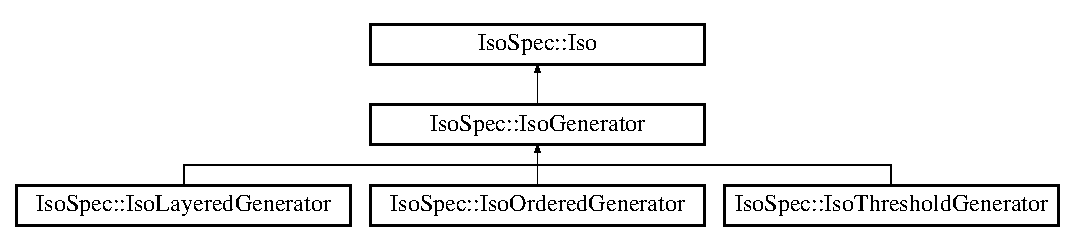
\includegraphics[height=2.800000cm]{class_iso_spec_1_1_iso}
\end{center}
\end{figure}
\subsection*{Public Member Functions}
\begin{DoxyCompactItemize}
\item 
\mbox{\hyperlink{class_iso_spec_1_1_iso_a5ff1fafd079a866e9d61bc7d859842ea}{Iso}} (int \+\_\+dim\+Number, const int $\ast$\+\_\+isotope\+Numbers, const int $\ast$\+\_\+atom\+Counts, const double $\ast$const $\ast$\+\_\+isotope\+Masses, const double $\ast$const $\ast$\+\_\+isotope\+Probabilities)
\begin{DoxyCompactList}\small\item\em General constructror. \end{DoxyCompactList}\item 
\mbox{\Hypertarget{class_iso_spec_1_1_iso_ad389effb319e9ed73db9ed5749868b81}\label{class_iso_spec_1_1_iso_ad389effb319e9ed73db9ed5749868b81}} 
\mbox{\hyperlink{class_iso_spec_1_1_iso_ad389effb319e9ed73db9ed5749868b81}{Iso}} (const char $\ast$formula)
\begin{DoxyCompactList}\small\item\em Constructor from the formula object. \end{DoxyCompactList}\item 
\mbox{\Hypertarget{class_iso_spec_1_1_iso_a6c93ecb77a11bc831cc7600797fbf837}\label{class_iso_spec_1_1_iso_a6c93ecb77a11bc831cc7600797fbf837}} 
\mbox{\hyperlink{class_iso_spec_1_1_iso_a6c93ecb77a11bc831cc7600797fbf837}{Iso}} (\mbox{\hyperlink{class_iso_spec_1_1_iso}{Iso}} \&\&other)
\begin{DoxyCompactList}\small\item\em The move constructor. \end{DoxyCompactList}\item 
\mbox{\hyperlink{class_iso_spec_1_1_iso_a485cba7555fbdc64bbea19690f202b13}{Iso}} (const \mbox{\hyperlink{class_iso_spec_1_1_iso}{Iso}} \&other, bool fullcopy)
\begin{DoxyCompactList}\small\item\em The copy constructor. \end{DoxyCompactList}\item 
\mbox{\Hypertarget{class_iso_spec_1_1_iso_a8cf8f90338bfc3e5117f5b491f7b523f}\label{class_iso_spec_1_1_iso_a8cf8f90338bfc3e5117f5b491f7b523f}} 
virtual \mbox{\hyperlink{class_iso_spec_1_1_iso_a8cf8f90338bfc3e5117f5b491f7b523f}{$\sim$\+Iso}} ()
\begin{DoxyCompactList}\small\item\em Destructor. \end{DoxyCompactList}\item 
\mbox{\Hypertarget{class_iso_spec_1_1_iso_a7541599fbc29dd374bb60e5eb8fc047d}\label{class_iso_spec_1_1_iso_a7541599fbc29dd374bb60e5eb8fc047d}} 
double \mbox{\hyperlink{class_iso_spec_1_1_iso_a7541599fbc29dd374bb60e5eb8fc047d}{get\+Lightest\+Peak\+Mass}} () const
\begin{DoxyCompactList}\small\item\em Get the mass of the lightest peak in the isotopic distribution. \end{DoxyCompactList}\item 
\mbox{\Hypertarget{class_iso_spec_1_1_iso_a1ede5e34e5bbbb22ae89b362ce2c6faf}\label{class_iso_spec_1_1_iso_a1ede5e34e5bbbb22ae89b362ce2c6faf}} 
double \mbox{\hyperlink{class_iso_spec_1_1_iso_a1ede5e34e5bbbb22ae89b362ce2c6faf}{get\+Heaviest\+Peak\+Mass}} () const
\begin{DoxyCompactList}\small\item\em Get the mass of the heaviest peak in the isotopic distribution. \end{DoxyCompactList}\item 
\mbox{\Hypertarget{class_iso_spec_1_1_iso_a9035d076cec8f937d971e3fd972aa83f}\label{class_iso_spec_1_1_iso_a9035d076cec8f937d971e3fd972aa83f}} 
double \mbox{\hyperlink{class_iso_spec_1_1_iso_a9035d076cec8f937d971e3fd972aa83f}{get\+Mode\+L\+Prob}} () const
\begin{DoxyCompactList}\small\item\em Get the log-\/probability of the mode-\/configuration (if there are many modes, they share this value). \end{DoxyCompactList}\item 
\mbox{\Hypertarget{class_iso_spec_1_1_iso_a62b17f48d86f62b5ed38ffb296a9daa5}\label{class_iso_spec_1_1_iso_a62b17f48d86f62b5ed38ffb296a9daa5}} 
int \mbox{\hyperlink{class_iso_spec_1_1_iso_a62b17f48d86f62b5ed38ffb296a9daa5}{get\+Dim\+Number}} () const
\begin{DoxyCompactList}\small\item\em Get the number of elements in the chemical formula of the molecule. \end{DoxyCompactList}\item 
\mbox{\Hypertarget{class_iso_spec_1_1_iso_a656a37dd84a6c0534b2373210ed5a091}\label{class_iso_spec_1_1_iso_a656a37dd84a6c0534b2373210ed5a091}} 
int \mbox{\hyperlink{class_iso_spec_1_1_iso_a656a37dd84a6c0534b2373210ed5a091}{get\+All\+Dim}} () const
\begin{DoxyCompactList}\small\item\em Get the total number of isotopes of elements present in a chemical formula. \end{DoxyCompactList}\end{DoxyCompactItemize}
\subsection*{Public Attributes}
\begin{DoxyCompactItemize}
\item 
bool \mbox{\hyperlink{class_iso_spec_1_1_iso_ad2a353f2c746648b08a9ad31ff775766}{disowned}}
\end{DoxyCompactItemize}
\subsection*{Protected Attributes}
\begin{DoxyCompactItemize}
\item 
int \mbox{\hyperlink{class_iso_spec_1_1_iso_a90245f9bc318f12720c134f61bbe0db0}{dim\+Number}}
\item 
int $\ast$ \mbox{\hyperlink{class_iso_spec_1_1_iso_a7235f0afc56dccd13937791a630c45da}{isotope\+Numbers}}
\item 
int $\ast$ \mbox{\hyperlink{class_iso_spec_1_1_iso_ab01939334b6c3e69f65a36f9965971a2}{atom\+Counts}}
\item 
unsigned int \mbox{\hyperlink{class_iso_spec_1_1_iso_a89ed144bf2495fa25840aca90a31b425}{conf\+Size}}
\item 
int \mbox{\hyperlink{class_iso_spec_1_1_iso_a8dd2c443706935b582979b13f935115c}{all\+Dim}}
\item 
\mbox{\hyperlink{class_iso_spec_1_1_marginal}{Marginal}} $\ast$$\ast$ \mbox{\hyperlink{class_iso_spec_1_1_iso_aea98a8331a2f8a1a6bbcace6124fcfae}{marginals}}
\item 
double \mbox{\hyperlink{class_iso_spec_1_1_iso_ab51c157b23ae6a6b521667b6f0e8a208}{mode\+L\+Prob}}
\end{DoxyCompactItemize}


\subsection{Detailed Description}
The \mbox{\hyperlink{class_iso_spec_1_1_iso}{Iso}} class for the calculation of the isotopic distribution. 

It contains full description of the molecule for which one would like to calculate the isotopic distribution. 

Definition at line 52 of file iso\+Spec++.\+h.



\subsection{Constructor \& Destructor Documentation}
\mbox{\Hypertarget{class_iso_spec_1_1_iso_a5ff1fafd079a866e9d61bc7d859842ea}\label{class_iso_spec_1_1_iso_a5ff1fafd079a866e9d61bc7d859842ea}} 
\index{Iso\+Spec\+::\+Iso@{Iso\+Spec\+::\+Iso}!Iso@{Iso}}
\index{Iso@{Iso}!Iso\+Spec\+::\+Iso@{Iso\+Spec\+::\+Iso}}
\subsubsection{\texorpdfstring{Iso()}{Iso()}\hspace{0.1cm}{\footnotesize\ttfamily [1/2]}}
{\footnotesize\ttfamily Iso\+Spec\+::\+Iso\+::\+Iso (\begin{DoxyParamCaption}\item[{int}]{\+\_\+dim\+Number,  }\item[{const int $\ast$}]{\+\_\+isotope\+Numbers,  }\item[{const int $\ast$}]{\+\_\+atom\+Counts,  }\item[{const double $\ast$const $\ast$}]{\+\_\+isotope\+Masses,  }\item[{const double $\ast$const $\ast$}]{\+\_\+isotope\+Probabilities }\end{DoxyParamCaption})}



General constructror. 


\begin{DoxyParams}{Parameters}
{\em \+\_\+dim\+Number} & The number of elements in the formula, e.\+g. for C100\+H202 it would be 2, as there are only carbon and hydrogen atoms. \\
\hline
{\em \+\_\+isotope\+Numbers} & A table with numbers of isotopes for each element, e.\+g. for C100\+H202 it would be \{2, 2\}, because both C and H have two stable isotopes. \\
\hline
{\em \+\_\+atom\+Counts} & Number of atoms of each element in the formula, e.\+g. for C100\+H202 corresponds to \{100, 202\}. \\
\hline
{\em \+\_\+isotope\+Masses} & A table of masses of isotopes of the elements in the chemical formula, e.\+g. \{12.\+0, 13.\+003355, 1.\+007825, 2.\+014102\} for C100\+H202. \\
\hline
{\em \+\_\+isotope\+Probabilities} & A table of isotope frequencies of the elements in the chemical formula, e.\+g. \{.989212, .010788, .999885, .000115\} for C100\+H202. \\
\hline
\end{DoxyParams}


Definition at line 51 of file iso\+Spec++.\+cpp.

\mbox{\Hypertarget{class_iso_spec_1_1_iso_a485cba7555fbdc64bbea19690f202b13}\label{class_iso_spec_1_1_iso_a485cba7555fbdc64bbea19690f202b13}} 
\index{Iso\+Spec\+::\+Iso@{Iso\+Spec\+::\+Iso}!Iso@{Iso}}
\index{Iso@{Iso}!Iso\+Spec\+::\+Iso@{Iso\+Spec\+::\+Iso}}
\subsubsection{\texorpdfstring{Iso()}{Iso()}\hspace{0.1cm}{\footnotesize\ttfamily [2/2]}}
{\footnotesize\ttfamily Iso\+Spec\+::\+Iso\+::\+Iso (\begin{DoxyParamCaption}\item[{const \mbox{\hyperlink{class_iso_spec_1_1_iso}{Iso}} \&}]{other,  }\item[{bool}]{fullcopy }\end{DoxyParamCaption})}



The copy constructor. 


\begin{DoxyParams}{Parameters}
{\em other} & The other instance of the \mbox{\hyperlink{class_iso_spec_1_1_iso}{Iso}} class. \\
\hline
{\em fullcopy} & If false, copy only the number of atoms in the formula, the size of the configuration, the total number of isotopes, and the probability of the mode isotopologue. \\
\hline
\end{DoxyParams}


Definition at line 84 of file iso\+Spec++.\+cpp.



\subsection{Member Data Documentation}
\mbox{\Hypertarget{class_iso_spec_1_1_iso_a8dd2c443706935b582979b13f935115c}\label{class_iso_spec_1_1_iso_a8dd2c443706935b582979b13f935115c}} 
\index{Iso\+Spec\+::\+Iso@{Iso\+Spec\+::\+Iso}!all\+Dim@{all\+Dim}}
\index{all\+Dim@{all\+Dim}!Iso\+Spec\+::\+Iso@{Iso\+Spec\+::\+Iso}}
\subsubsection{\texorpdfstring{all\+Dim}{allDim}}
{\footnotesize\ttfamily int Iso\+Spec\+::\+Iso\+::all\+Dim\hspace{0.3cm}{\ttfamily [protected]}}

The total number of isotopes of elements present in a chemical formula, e.\+g. for H20 it is 2+3=5. 

Definition at line 71 of file iso\+Spec++.\+h.

\mbox{\Hypertarget{class_iso_spec_1_1_iso_ab01939334b6c3e69f65a36f9965971a2}\label{class_iso_spec_1_1_iso_ab01939334b6c3e69f65a36f9965971a2}} 
\index{Iso\+Spec\+::\+Iso@{Iso\+Spec\+::\+Iso}!atom\+Counts@{atom\+Counts}}
\index{atom\+Counts@{atom\+Counts}!Iso\+Spec\+::\+Iso@{Iso\+Spec\+::\+Iso}}
\subsubsection{\texorpdfstring{atom\+Counts}{atomCounts}}
{\footnotesize\ttfamily int$\ast$ Iso\+Spec\+::\+Iso\+::atom\+Counts\hspace{0.3cm}{\ttfamily [protected]}}

A table with numbers of isotopes for each element. 

Definition at line 69 of file iso\+Spec++.\+h.

\mbox{\Hypertarget{class_iso_spec_1_1_iso_a89ed144bf2495fa25840aca90a31b425}\label{class_iso_spec_1_1_iso_a89ed144bf2495fa25840aca90a31b425}} 
\index{Iso\+Spec\+::\+Iso@{Iso\+Spec\+::\+Iso}!conf\+Size@{conf\+Size}}
\index{conf\+Size@{conf\+Size}!Iso\+Spec\+::\+Iso@{Iso\+Spec\+::\+Iso}}
\subsubsection{\texorpdfstring{conf\+Size}{confSize}}
{\footnotesize\ttfamily unsigned int Iso\+Spec\+::\+Iso\+::conf\+Size\hspace{0.3cm}{\ttfamily [protected]}}

The number of bytes needed to represent the counts of isotopes present in the extended chemical formula. 

Definition at line 70 of file iso\+Spec++.\+h.

\mbox{\Hypertarget{class_iso_spec_1_1_iso_a90245f9bc318f12720c134f61bbe0db0}\label{class_iso_spec_1_1_iso_a90245f9bc318f12720c134f61bbe0db0}} 
\index{Iso\+Spec\+::\+Iso@{Iso\+Spec\+::\+Iso}!dim\+Number@{dim\+Number}}
\index{dim\+Number@{dim\+Number}!Iso\+Spec\+::\+Iso@{Iso\+Spec\+::\+Iso}}
\subsubsection{\texorpdfstring{dim\+Number}{dimNumber}}
{\footnotesize\ttfamily int Iso\+Spec\+::\+Iso\+::dim\+Number\hspace{0.3cm}{\ttfamily [protected]}}

The number of elements in the chemical formula of the molecule. 

Definition at line 67 of file iso\+Spec++.\+h.

\mbox{\Hypertarget{class_iso_spec_1_1_iso_ad2a353f2c746648b08a9ad31ff775766}\label{class_iso_spec_1_1_iso_ad2a353f2c746648b08a9ad31ff775766}} 
\index{Iso\+Spec\+::\+Iso@{Iso\+Spec\+::\+Iso}!disowned@{disowned}}
\index{disowned@{disowned}!Iso\+Spec\+::\+Iso@{Iso\+Spec\+::\+Iso}}
\subsubsection{\texorpdfstring{disowned}{disowned}}
{\footnotesize\ttfamily bool Iso\+Spec\+::\+Iso\+::disowned}

A variable showing if the \mbox{\hyperlink{class_iso_spec_1_1_iso}{Iso}} class was specialized by its child-\/class. If so, then the description of the molecules has been transfered there and \mbox{\hyperlink{class_iso_spec_1_1_iso}{Iso}} is a carcass class, dead as a dodo, an ex-\/class if you will. 

Definition at line 65 of file iso\+Spec++.\+h.

\mbox{\Hypertarget{class_iso_spec_1_1_iso_a7235f0afc56dccd13937791a630c45da}\label{class_iso_spec_1_1_iso_a7235f0afc56dccd13937791a630c45da}} 
\index{Iso\+Spec\+::\+Iso@{Iso\+Spec\+::\+Iso}!isotope\+Numbers@{isotope\+Numbers}}
\index{isotope\+Numbers@{isotope\+Numbers}!Iso\+Spec\+::\+Iso@{Iso\+Spec\+::\+Iso}}
\subsubsection{\texorpdfstring{isotope\+Numbers}{isotopeNumbers}}
{\footnotesize\ttfamily int$\ast$ Iso\+Spec\+::\+Iso\+::isotope\+Numbers\hspace{0.3cm}{\ttfamily [protected]}}

A table with numbers of isotopes for each element. 

Definition at line 68 of file iso\+Spec++.\+h.

\mbox{\Hypertarget{class_iso_spec_1_1_iso_aea98a8331a2f8a1a6bbcace6124fcfae}\label{class_iso_spec_1_1_iso_aea98a8331a2f8a1a6bbcace6124fcfae}} 
\index{Iso\+Spec\+::\+Iso@{Iso\+Spec\+::\+Iso}!marginals@{marginals}}
\index{marginals@{marginals}!Iso\+Spec\+::\+Iso@{Iso\+Spec\+::\+Iso}}
\subsubsection{\texorpdfstring{marginals}{marginals}}
{\footnotesize\ttfamily \mbox{\hyperlink{class_iso_spec_1_1_marginal}{Marginal}}$\ast$$\ast$ Iso\+Spec\+::\+Iso\+::marginals\hspace{0.3cm}{\ttfamily [protected]}}

The table of pointers to the distributions of individual subisotopologues. 

Definition at line 72 of file iso\+Spec++.\+h.

\mbox{\Hypertarget{class_iso_spec_1_1_iso_ab51c157b23ae6a6b521667b6f0e8a208}\label{class_iso_spec_1_1_iso_ab51c157b23ae6a6b521667b6f0e8a208}} 
\index{Iso\+Spec\+::\+Iso@{Iso\+Spec\+::\+Iso}!mode\+L\+Prob@{mode\+L\+Prob}}
\index{mode\+L\+Prob@{mode\+L\+Prob}!Iso\+Spec\+::\+Iso@{Iso\+Spec\+::\+Iso}}
\subsubsection{\texorpdfstring{mode\+L\+Prob}{modeLProb}}
{\footnotesize\ttfamily double Iso\+Spec\+::\+Iso\+::mode\+L\+Prob\hspace{0.3cm}{\ttfamily [protected]}}

The log-\/probability of the mode of the isotopic distribution. 

Definition at line 73 of file iso\+Spec++.\+h.



The documentation for this class was generated from the following files\+:\begin{DoxyCompactItemize}
\item 
/\+Users/matteo/\+Projects/isospec/\+Iso\+Spec/\+Iso\+Spec++/iso\+Spec++.\+h\item 
/\+Users/matteo/\+Projects/isospec/\+Iso\+Spec/\+Iso\+Spec++/iso\+Spec++.\+cpp\end{DoxyCompactItemize}

\hypertarget{class_iso_spec_1_1_iso_generator}{}\section{Iso\+Spec\+:\+:Iso\+Generator Class Reference}
\label{class_iso_spec_1_1_iso_generator}\index{Iso\+Spec\+::\+Iso\+Generator@{Iso\+Spec\+::\+Iso\+Generator}}


The generator of isotopologues.  




{\ttfamily \#include $<$iso\+Spec++.\+h$>$}

Inheritance diagram for Iso\+Spec\+:\+:Iso\+Generator\+:\begin{figure}[H]
\begin{center}
\leavevmode
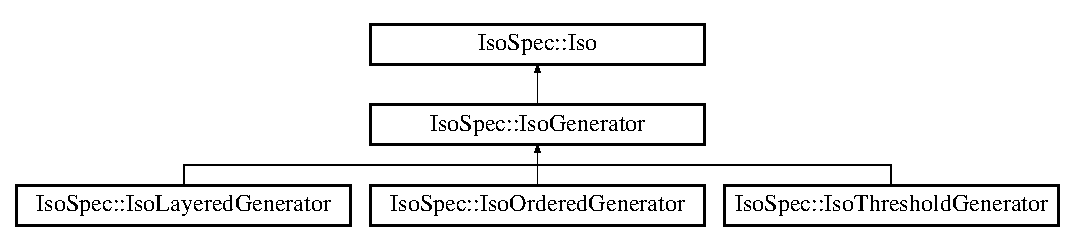
\includegraphics[height=2.800000cm]{class_iso_spec_1_1_iso_generator}
\end{center}
\end{figure}
\subsection*{Public Member Functions}
\begin{DoxyCompactItemize}
\item 
virtual bool \mbox{\hyperlink{class_iso_spec_1_1_iso_generator_a20f48ba18c6aecc57d73b2c3ec3a11dd}{advance\+To\+Next\+Configuration}} ()=0
\begin{DoxyCompactList}\small\item\em Advance to the next, not yet visited, most probable isotopologue. \end{DoxyCompactList}\item 
virtual double \mbox{\hyperlink{class_iso_spec_1_1_iso_generator_ae8e24abbce51a4c93994f630acfdf383}{lprob}} () const
\begin{DoxyCompactList}\small\item\em Get the log-\/probability of the current isotopologue. \end{DoxyCompactList}\item 
virtual double \mbox{\hyperlink{class_iso_spec_1_1_iso_generator_a34173228ef73e272e2ff0ae6ce58092d}{mass}} () const
\begin{DoxyCompactList}\small\item\em Get the mass of the current isotopologue. \end{DoxyCompactList}\item 
virtual double \mbox{\hyperlink{class_iso_spec_1_1_iso_generator_aecf1b3292fcc0857a86efe619a37fff0}{prob}} () const
\begin{DoxyCompactList}\small\item\em Get the probability of the current isotopologue. \end{DoxyCompactList}\item 
\mbox{\Hypertarget{class_iso_spec_1_1_iso_generator_a19ca8af7dd97f8f37756d4267d49d91d}\label{class_iso_spec_1_1_iso_generator_a19ca8af7dd97f8f37756d4267d49d91d}} 
virtual void {\bfseries get\+\_\+conf\+\_\+signature} (int $\ast$space) const =0
\item 
\mbox{\Hypertarget{class_iso_spec_1_1_iso_generator_a89b5b851fbc67f79ed165af0b9b2a188}\label{class_iso_spec_1_1_iso_generator_a89b5b851fbc67f79ed165af0b9b2a188}} 
\mbox{\hyperlink{class_iso_spec_1_1_iso_generator_a89b5b851fbc67f79ed165af0b9b2a188}{Iso\+Generator}} (\mbox{\hyperlink{class_iso_spec_1_1_iso}{Iso}} \&\&iso, bool alloc\+\_\+partials=true)
\begin{DoxyCompactList}\small\item\em Move constructor. \end{DoxyCompactList}\item 
\mbox{\Hypertarget{class_iso_spec_1_1_iso_generator_a28442c8072a2e85faf5ff04f5feffd76}\label{class_iso_spec_1_1_iso_generator_a28442c8072a2e85faf5ff04f5feffd76}} 
virtual \mbox{\hyperlink{class_iso_spec_1_1_iso_generator_a28442c8072a2e85faf5ff04f5feffd76}{$\sim$\+Iso\+Generator}} ()
\begin{DoxyCompactList}\small\item\em Destructor. \end{DoxyCompactList}\end{DoxyCompactItemize}
\subsection*{Protected Attributes}
\begin{DoxyCompactItemize}
\item 
double $\ast$ \mbox{\hyperlink{class_iso_spec_1_1_iso_generator_a54a39b847a71aa08d1207d0666dd62bc}{partial\+L\+Probs}}
\item 
double $\ast$ \mbox{\hyperlink{class_iso_spec_1_1_iso_generator_af5654fcdba8199cbd60668af5de89a53}{partial\+Masses}}
\item 
double $\ast$ \mbox{\hyperlink{class_iso_spec_1_1_iso_generator_ac18406df84b4b220bcb1974000c192b2}{partial\+Probs}}
\end{DoxyCompactItemize}
\subsection*{Additional Inherited Members}


\subsection{Detailed Description}
The generator of isotopologues. 

This class provides the common interface for all isotopic generators. 

Definition at line 129 of file iso\+Spec++.\+h.



\subsection{Member Function Documentation}
\mbox{\Hypertarget{class_iso_spec_1_1_iso_generator_a20f48ba18c6aecc57d73b2c3ec3a11dd}\label{class_iso_spec_1_1_iso_generator_a20f48ba18c6aecc57d73b2c3ec3a11dd}} 
\index{Iso\+Spec\+::\+Iso\+Generator@{Iso\+Spec\+::\+Iso\+Generator}!advance\+To\+Next\+Configuration@{advance\+To\+Next\+Configuration}}
\index{advance\+To\+Next\+Configuration@{advance\+To\+Next\+Configuration}!Iso\+Spec\+::\+Iso\+Generator@{Iso\+Spec\+::\+Iso\+Generator}}
\subsubsection{\texorpdfstring{advance\+To\+Next\+Configuration()}{advanceToNextConfiguration()}}
{\footnotesize\ttfamily virtual bool Iso\+Spec\+::\+Iso\+Generator\+::advance\+To\+Next\+Configuration (\begin{DoxyParamCaption}{ }\end{DoxyParamCaption})\hspace{0.3cm}{\ttfamily [pure virtual]}}



Advance to the next, not yet visited, most probable isotopologue. 

\begin{DoxyReturn}{Returns}
Return false if it is not possible to advance. 
\end{DoxyReturn}


Implemented in \mbox{\hyperlink{class_iso_spec_1_1_iso_layered_generator_abce0871ac279fd54a0344ceb80126b66}{Iso\+Spec\+::\+Iso\+Layered\+Generator}}, \mbox{\hyperlink{class_iso_spec_1_1_iso_threshold_generator_a7164a6476b84665967c4a667a91d3f3e}{Iso\+Spec\+::\+Iso\+Threshold\+Generator}}, and \mbox{\hyperlink{class_iso_spec_1_1_iso_ordered_generator_aa2438bb81fb1d68eda1637d67e9cb36d}{Iso\+Spec\+::\+Iso\+Ordered\+Generator}}.

\mbox{\Hypertarget{class_iso_spec_1_1_iso_generator_ae8e24abbce51a4c93994f630acfdf383}\label{class_iso_spec_1_1_iso_generator_ae8e24abbce51a4c93994f630acfdf383}} 
\index{Iso\+Spec\+::\+Iso\+Generator@{Iso\+Spec\+::\+Iso\+Generator}!lprob@{lprob}}
\index{lprob@{lprob}!Iso\+Spec\+::\+Iso\+Generator@{Iso\+Spec\+::\+Iso\+Generator}}
\subsubsection{\texorpdfstring{lprob()}{lprob()}}
{\footnotesize\ttfamily virtual double Iso\+Spec\+::\+Iso\+Generator\+::lprob (\begin{DoxyParamCaption}{ }\end{DoxyParamCaption}) const\hspace{0.3cm}{\ttfamily [inline]}, {\ttfamily [virtual]}}



Get the log-\/probability of the current isotopologue. 

\begin{DoxyReturn}{Returns}
The log-\/probability of the current isotopologue. 
\end{DoxyReturn}


Reimplemented in \mbox{\hyperlink{class_iso_spec_1_1_iso_threshold_generator_a4aeebde03e385404d0175fd5696ff529}{Iso\+Spec\+::\+Iso\+Threshold\+Generator}}.



Definition at line 147 of file iso\+Spec++.\+h.

\mbox{\Hypertarget{class_iso_spec_1_1_iso_generator_a34173228ef73e272e2ff0ae6ce58092d}\label{class_iso_spec_1_1_iso_generator_a34173228ef73e272e2ff0ae6ce58092d}} 
\index{Iso\+Spec\+::\+Iso\+Generator@{Iso\+Spec\+::\+Iso\+Generator}!mass@{mass}}
\index{mass@{mass}!Iso\+Spec\+::\+Iso\+Generator@{Iso\+Spec\+::\+Iso\+Generator}}
\subsubsection{\texorpdfstring{mass()}{mass()}}
{\footnotesize\ttfamily virtual double Iso\+Spec\+::\+Iso\+Generator\+::mass (\begin{DoxyParamCaption}{ }\end{DoxyParamCaption}) const\hspace{0.3cm}{\ttfamily [inline]}, {\ttfamily [virtual]}}



Get the mass of the current isotopologue. 

\begin{DoxyReturn}{Returns}
The mass of the current isotopologue. 
\end{DoxyReturn}


Reimplemented in \mbox{\hyperlink{class_iso_spec_1_1_iso_threshold_generator_ae2236accc7dc7a25a723e3c7317659b6}{Iso\+Spec\+::\+Iso\+Threshold\+Generator}}.



Definition at line 153 of file iso\+Spec++.\+h.

\mbox{\Hypertarget{class_iso_spec_1_1_iso_generator_aecf1b3292fcc0857a86efe619a37fff0}\label{class_iso_spec_1_1_iso_generator_aecf1b3292fcc0857a86efe619a37fff0}} 
\index{Iso\+Spec\+::\+Iso\+Generator@{Iso\+Spec\+::\+Iso\+Generator}!prob@{prob}}
\index{prob@{prob}!Iso\+Spec\+::\+Iso\+Generator@{Iso\+Spec\+::\+Iso\+Generator}}
\subsubsection{\texorpdfstring{prob()}{prob()}}
{\footnotesize\ttfamily virtual double Iso\+Spec\+::\+Iso\+Generator\+::prob (\begin{DoxyParamCaption}{ }\end{DoxyParamCaption}) const\hspace{0.3cm}{\ttfamily [inline]}, {\ttfamily [virtual]}}



Get the probability of the current isotopologue. 

\begin{DoxyReturn}{Returns}
The probability of the current isotopologue. 
\end{DoxyReturn}


Reimplemented in \mbox{\hyperlink{class_iso_spec_1_1_iso_threshold_generator_a998d987f81b2ca7ed610294f6a5f8df5}{Iso\+Spec\+::\+Iso\+Threshold\+Generator}}.



Definition at line 159 of file iso\+Spec++.\+h.



\subsection{Member Data Documentation}
\mbox{\Hypertarget{class_iso_spec_1_1_iso_generator_a54a39b847a71aa08d1207d0666dd62bc}\label{class_iso_spec_1_1_iso_generator_a54a39b847a71aa08d1207d0666dd62bc}} 
\index{Iso\+Spec\+::\+Iso\+Generator@{Iso\+Spec\+::\+Iso\+Generator}!partial\+L\+Probs@{partial\+L\+Probs}}
\index{partial\+L\+Probs@{partial\+L\+Probs}!Iso\+Spec\+::\+Iso\+Generator@{Iso\+Spec\+::\+Iso\+Generator}}
\subsubsection{\texorpdfstring{partial\+L\+Probs}{partialLProbs}}
{\footnotesize\ttfamily double$\ast$ Iso\+Spec\+::\+Iso\+Generator\+::partial\+L\+Probs\hspace{0.3cm}{\ttfamily [protected]}}

The prefix sum of the log-\/probabilities of the current isotopologue. 

Definition at line 132 of file iso\+Spec++.\+h.

\mbox{\Hypertarget{class_iso_spec_1_1_iso_generator_af5654fcdba8199cbd60668af5de89a53}\label{class_iso_spec_1_1_iso_generator_af5654fcdba8199cbd60668af5de89a53}} 
\index{Iso\+Spec\+::\+Iso\+Generator@{Iso\+Spec\+::\+Iso\+Generator}!partial\+Masses@{partial\+Masses}}
\index{partial\+Masses@{partial\+Masses}!Iso\+Spec\+::\+Iso\+Generator@{Iso\+Spec\+::\+Iso\+Generator}}
\subsubsection{\texorpdfstring{partial\+Masses}{partialMasses}}
{\footnotesize\ttfamily double$\ast$ Iso\+Spec\+::\+Iso\+Generator\+::partial\+Masses\hspace{0.3cm}{\ttfamily [protected]}}

The prefix sum of the masses of the current isotopologue. 

Definition at line 133 of file iso\+Spec++.\+h.

\mbox{\Hypertarget{class_iso_spec_1_1_iso_generator_ac18406df84b4b220bcb1974000c192b2}\label{class_iso_spec_1_1_iso_generator_ac18406df84b4b220bcb1974000c192b2}} 
\index{Iso\+Spec\+::\+Iso\+Generator@{Iso\+Spec\+::\+Iso\+Generator}!partial\+Probs@{partial\+Probs}}
\index{partial\+Probs@{partial\+Probs}!Iso\+Spec\+::\+Iso\+Generator@{Iso\+Spec\+::\+Iso\+Generator}}
\subsubsection{\texorpdfstring{partial\+Probs}{partialProbs}}
{\footnotesize\ttfamily double$\ast$ Iso\+Spec\+::\+Iso\+Generator\+::partial\+Probs\hspace{0.3cm}{\ttfamily [protected]}}

The prefix product of the probabilities of the current isotopologue. 

Definition at line 134 of file iso\+Spec++.\+h.



The documentation for this class was generated from the following files\+:\begin{DoxyCompactItemize}
\item 
/\+Users/matteo/\+Projects/isospec/\+Iso\+Spec/\+Iso\+Spec++/iso\+Spec++.\+h\item 
/\+Users/matteo/\+Projects/isospec/\+Iso\+Spec/\+Iso\+Spec++/iso\+Spec++.\+cpp\end{DoxyCompactItemize}

\hypertarget{class_iso_spec_1_1_iso_layered_generator}{}\section{Iso\+Spec\+:\+:Iso\+Layered\+Generator Class Reference}
\label{class_iso_spec_1_1_iso_layered_generator}\index{Iso\+Spec\+::\+Iso\+Layered\+Generator@{Iso\+Spec\+::\+Iso\+Layered\+Generator}}


The class that represents isotopologues above a given joint probability value.  




{\ttfamily \#include $<$iso\+Spec++.\+h$>$}

Inheritance diagram for Iso\+Spec\+:\+:Iso\+Layered\+Generator\+:\begin{figure}[H]
\begin{center}
\leavevmode
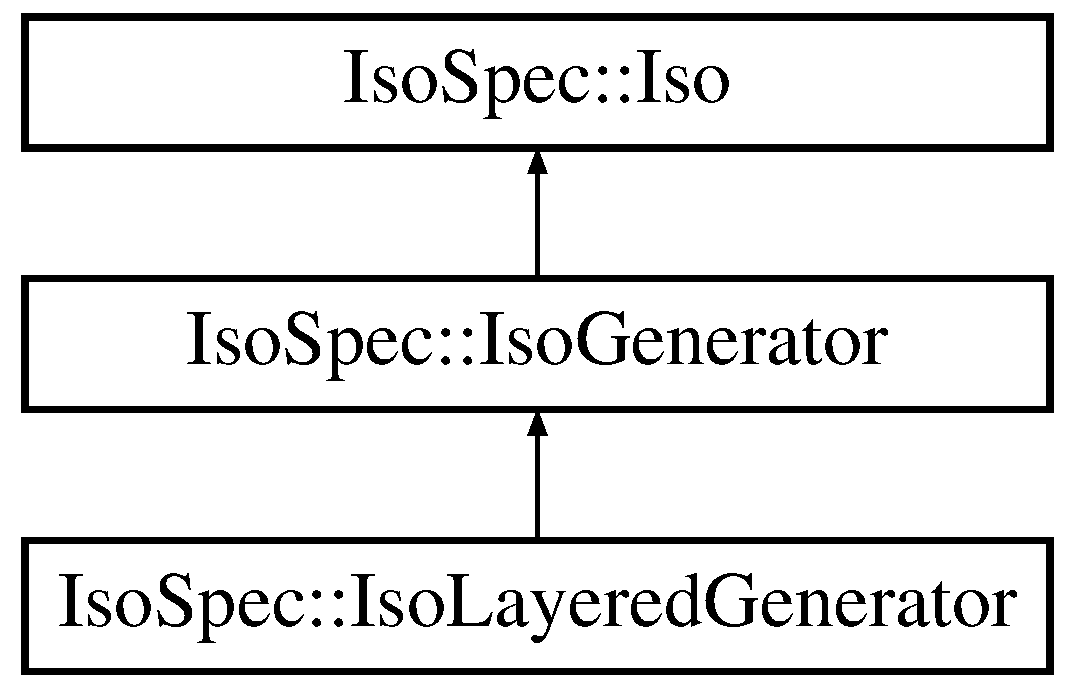
\includegraphics[height=3.000000cm]{class_iso_spec_1_1_iso_layered_generator}
\end{center}
\end{figure}
\subsection*{Public Member Functions}
\begin{DoxyCompactItemize}
\item 
bool \mbox{\hyperlink{class_iso_spec_1_1_iso_layered_generator_abce0871ac279fd54a0344ceb80126b66}{advance\+To\+Next\+Configuration}} () override final
\begin{DoxyCompactList}\small\item\em Advance to the next, not yet visited, most probable isotopologue. \end{DoxyCompactList}\item 
\mbox{\Hypertarget{class_iso_spec_1_1_iso_layered_generator_ab63cbae392f88528e5b7421dada4abef}\label{class_iso_spec_1_1_iso_layered_generator_ab63cbae392f88528e5b7421dada4abef}} 
void {\bfseries get\+\_\+conf\+\_\+signature} (int $\ast$space) const override final
\item 
\mbox{\Hypertarget{class_iso_spec_1_1_iso_layered_generator_a746fc9fe13cca843a0f0f1993aee970a}\label{class_iso_spec_1_1_iso_layered_generator_a746fc9fe13cca843a0f0f1993aee970a}} 
{\bfseries Iso\+Layered\+Generator} (\mbox{\hyperlink{class_iso_spec_1_1_iso}{Iso}} \&\&iso, double \+\_\+target\+Coverage, double \+\_\+percentage\+To\+Expand, int \+\_\+tab\+Size=1000, int \+\_\+hash\+Size=1000, bool trim=false)
\item 
\mbox{\Hypertarget{class_iso_spec_1_1_iso_layered_generator_a6c4ea5906136d802859f47cd1b5add8d}\label{class_iso_spec_1_1_iso_layered_generator_a6c4ea5906136d802859f47cd1b5add8d}} 
void {\bfseries terminate\+\_\+search} ()
\end{DoxyCompactItemize}
\subsection*{Additional Inherited Members}


\subsection{Detailed Description}
The class that represents isotopologues above a given joint probability value. 

This class generates subsequent isotopologues that A\+RE N\+OT G\+U\+A\+R\+A\+N\+T\+E\+ED TO BE O\+R\+D\+E\+R\+ED BY probability. The overal set of isotopologues is guaranteed to surpass a given threshold of probability contained in the isotopic distribution. This calculations are performed in O(\+N) operations, where N is the total number of the output isotopologues.

This class is not a true generator yet -\/ the generator methods have been implemented for compatibility, but the class actually performs all computations during the initialization and stores them, and the generator methods only walk through the array of precomputed values. . It will be reimplemented as a true generator in 2.\+0. 

Definition at line 383 of file iso\+Spec++.\+h.



\subsection{Member Function Documentation}
\mbox{\Hypertarget{class_iso_spec_1_1_iso_layered_generator_abce0871ac279fd54a0344ceb80126b66}\label{class_iso_spec_1_1_iso_layered_generator_abce0871ac279fd54a0344ceb80126b66}} 
\index{Iso\+Spec\+::\+Iso\+Layered\+Generator@{Iso\+Spec\+::\+Iso\+Layered\+Generator}!advance\+To\+Next\+Configuration@{advance\+To\+Next\+Configuration}}
\index{advance\+To\+Next\+Configuration@{advance\+To\+Next\+Configuration}!Iso\+Spec\+::\+Iso\+Layered\+Generator@{Iso\+Spec\+::\+Iso\+Layered\+Generator}}
\subsubsection{\texorpdfstring{advance\+To\+Next\+Configuration()}{advanceToNextConfiguration()}}
{\footnotesize\ttfamily bool Iso\+Spec\+::\+Iso\+Layered\+Generator\+::advance\+To\+Next\+Configuration (\begin{DoxyParamCaption}{ }\end{DoxyParamCaption})\hspace{0.3cm}{\ttfamily [final]}, {\ttfamily [override]}, {\ttfamily [virtual]}}



Advance to the next, not yet visited, most probable isotopologue. 

\begin{DoxyReturn}{Returns}
Return false if it is not possible to advance. 
\end{DoxyReturn}


Implements \mbox{\hyperlink{class_iso_spec_1_1_iso_generator_a20f48ba18c6aecc57d73b2c3ec3a11dd}{Iso\+Spec\+::\+Iso\+Generator}}.



Definition at line 773 of file iso\+Spec++.\+cpp.



The documentation for this class was generated from the following files\+:\begin{DoxyCompactItemize}
\item 
/\+Users/matteo/\+Projects/isospec/\+Iso\+Spec/\+Iso\+Spec++/iso\+Spec++.\+h\item 
/\+Users/matteo/\+Projects/isospec/\+Iso\+Spec/\+Iso\+Spec++/iso\+Spec++.\+cpp\end{DoxyCompactItemize}

\hypertarget{class_iso_spec_1_1_iso_ordered_generator}{}\section{Iso\+Spec\+:\+:Iso\+Ordered\+Generator Class Reference}
\label{class_iso_spec_1_1_iso_ordered_generator}\index{Iso\+Spec\+::\+Iso\+Ordered\+Generator@{Iso\+Spec\+::\+Iso\+Ordered\+Generator}}


The generator of isotopologues sorted by their probability of occurrence.  




{\ttfamily \#include $<$iso\+Spec++.\+h$>$}

Inheritance diagram for Iso\+Spec\+:\+:Iso\+Ordered\+Generator\+:\begin{figure}[H]
\begin{center}
\leavevmode
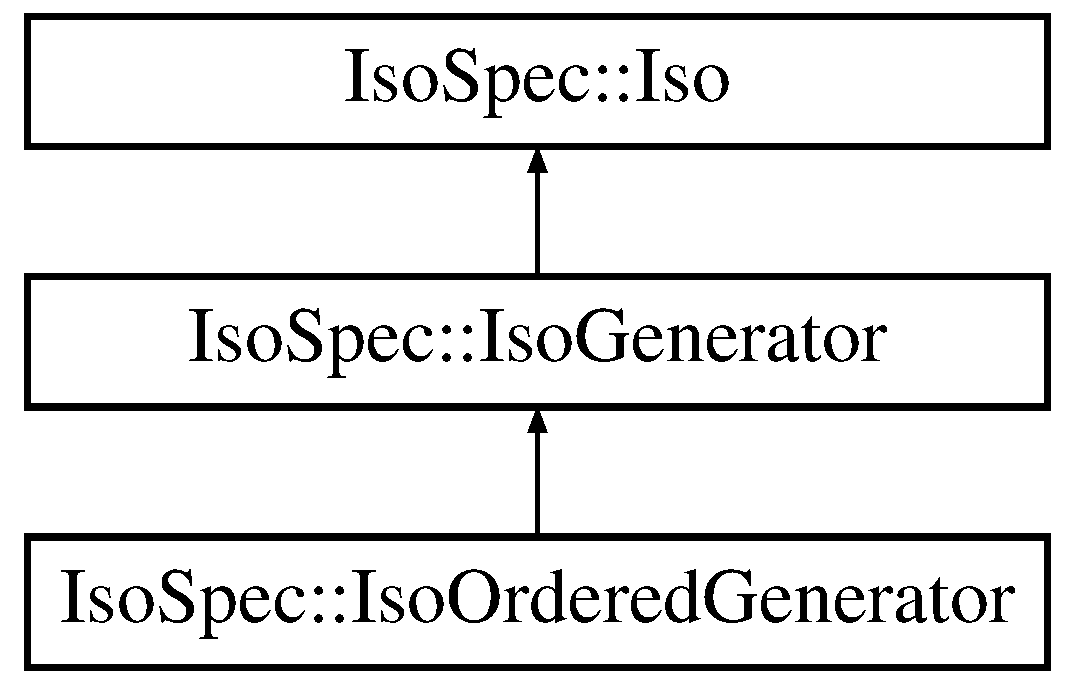
\includegraphics[height=3.000000cm]{class_iso_spec_1_1_iso_ordered_generator}
\end{center}
\end{figure}
\subsection*{Public Member Functions}
\begin{DoxyCompactItemize}
\item 
bool \mbox{\hyperlink{class_iso_spec_1_1_iso_ordered_generator_aa2438bb81fb1d68eda1637d67e9cb36d}{advance\+To\+Next\+Configuration}} () override final
\begin{DoxyCompactList}\small\item\em Advance to the next, not yet visited, most probable isotopologue. \end{DoxyCompactList}\item 
void \mbox{\hyperlink{class_iso_spec_1_1_iso_ordered_generator_af5d638985fd24c03bfe1f3d61e1b25c6}{get\+\_\+conf\+\_\+signature}} (int $\ast$space) const override final
\begin{DoxyCompactList}\small\item\em Save the counts of isotopes in the space. \end{DoxyCompactList}\item 
\mbox{\Hypertarget{class_iso_spec_1_1_iso_ordered_generator_afaf81ff3a758cd59629db323560e263d}\label{class_iso_spec_1_1_iso_ordered_generator_afaf81ff3a758cd59629db323560e263d}} 
\mbox{\hyperlink{class_iso_spec_1_1_iso_ordered_generator_afaf81ff3a758cd59629db323560e263d}{Iso\+Ordered\+Generator}} (\mbox{\hyperlink{class_iso_spec_1_1_iso}{Iso}} \&\&iso, int \+\_\+tab\+Size=1000, int \+\_\+hash\+Size=1000)
\begin{DoxyCompactList}\small\item\em The move-\/contstructor. \end{DoxyCompactList}\item 
\mbox{\Hypertarget{class_iso_spec_1_1_iso_ordered_generator_a030c118b9a6131130684cd2710371842}\label{class_iso_spec_1_1_iso_ordered_generator_a030c118b9a6131130684cd2710371842}} 
virtual \mbox{\hyperlink{class_iso_spec_1_1_iso_ordered_generator_a030c118b9a6131130684cd2710371842}{$\sim$\+Iso\+Ordered\+Generator}} ()
\begin{DoxyCompactList}\small\item\em Destructor. \end{DoxyCompactList}\end{DoxyCompactItemize}
\subsection*{Additional Inherited Members}


\subsection{Detailed Description}
The generator of isotopologues sorted by their probability of occurrence. 

The subsequent isotopologues are generated with diminishing probability, starting from the mode. This algorithm take O(\+N$\ast$log(\+N)) to compute the N isotopologues because of using the Priority Queue data structure. Obtaining the N isotopologues can be achieved in O(\+N) if they are not required to be spit out in the descending order. 

Definition at line 179 of file iso\+Spec++.\+h.



\subsection{Member Function Documentation}
\mbox{\Hypertarget{class_iso_spec_1_1_iso_ordered_generator_aa2438bb81fb1d68eda1637d67e9cb36d}\label{class_iso_spec_1_1_iso_ordered_generator_aa2438bb81fb1d68eda1637d67e9cb36d}} 
\index{Iso\+Spec\+::\+Iso\+Ordered\+Generator@{Iso\+Spec\+::\+Iso\+Ordered\+Generator}!advance\+To\+Next\+Configuration@{advance\+To\+Next\+Configuration}}
\index{advance\+To\+Next\+Configuration@{advance\+To\+Next\+Configuration}!Iso\+Spec\+::\+Iso\+Ordered\+Generator@{Iso\+Spec\+::\+Iso\+Ordered\+Generator}}
\subsubsection{\texorpdfstring{advance\+To\+Next\+Configuration()}{advanceToNextConfiguration()}}
{\footnotesize\ttfamily bool Iso\+Spec\+::\+Iso\+Ordered\+Generator\+::advance\+To\+Next\+Configuration (\begin{DoxyParamCaption}{ }\end{DoxyParamCaption})\hspace{0.3cm}{\ttfamily [final]}, {\ttfamily [override]}, {\ttfamily [virtual]}}



Advance to the next, not yet visited, most probable isotopologue. 

\begin{DoxyReturn}{Returns}
Return false if it is not possible to advance. 
\end{DoxyReturn}


Implements \mbox{\hyperlink{class_iso_spec_1_1_iso_generator_a20f48ba18c6aecc57d73b2c3ec3a11dd}{Iso\+Spec\+::\+Iso\+Generator}}.



Definition at line 461 of file iso\+Spec++.\+cpp.

\mbox{\Hypertarget{class_iso_spec_1_1_iso_ordered_generator_af5d638985fd24c03bfe1f3d61e1b25c6}\label{class_iso_spec_1_1_iso_ordered_generator_af5d638985fd24c03bfe1f3d61e1b25c6}} 
\index{Iso\+Spec\+::\+Iso\+Ordered\+Generator@{Iso\+Spec\+::\+Iso\+Ordered\+Generator}!get\+\_\+conf\+\_\+signature@{get\+\_\+conf\+\_\+signature}}
\index{get\+\_\+conf\+\_\+signature@{get\+\_\+conf\+\_\+signature}!Iso\+Spec\+::\+Iso\+Ordered\+Generator@{Iso\+Spec\+::\+Iso\+Ordered\+Generator}}
\subsubsection{\texorpdfstring{get\+\_\+conf\+\_\+signature()}{get\_conf\_signature()}}
{\footnotesize\ttfamily void Iso\+Spec\+::\+Iso\+Ordered\+Generator\+::get\+\_\+conf\+\_\+signature (\begin{DoxyParamCaption}\item[{int $\ast$}]{space }\end{DoxyParamCaption}) const\hspace{0.3cm}{\ttfamily [inline]}, {\ttfamily [final]}, {\ttfamily [override]}, {\ttfamily [virtual]}}



Save the counts of isotopes in the space. 


\begin{DoxyParams}{Parameters}
{\em space} & An array where counts of isotopes shall be written. Must be as big as the overall number of isotopes. \\
\hline
\end{DoxyParams}


Implements \mbox{\hyperlink{class_iso_spec_1_1_iso_generator}{Iso\+Spec\+::\+Iso\+Generator}}.



Definition at line 202 of file iso\+Spec++.\+h.



The documentation for this class was generated from the following files\+:\begin{DoxyCompactItemize}
\item 
/\+Users/matteo/\+Projects/isospec/\+Iso\+Spec/\+Iso\+Spec++/iso\+Spec++.\+h\item 
/\+Users/matteo/\+Projects/isospec/\+Iso\+Spec/\+Iso\+Spec++/iso\+Spec++.\+cpp\end{DoxyCompactItemize}

\hypertarget{class_iso_spec_1_1_iso_threshold_generator}{}\section{Iso\+Spec\+:\+:Iso\+Threshold\+Generator Class Reference}
\label{class_iso_spec_1_1_iso_threshold_generator}\index{Iso\+Spec\+::\+Iso\+Threshold\+Generator@{Iso\+Spec\+::\+Iso\+Threshold\+Generator}}


The generator of isotopologues above a given threshold value.  




{\ttfamily \#include $<$iso\+Spec++.\+h$>$}

Inheritance diagram for Iso\+Spec\+:\+:Iso\+Threshold\+Generator\+:\begin{figure}[H]
\begin{center}
\leavevmode
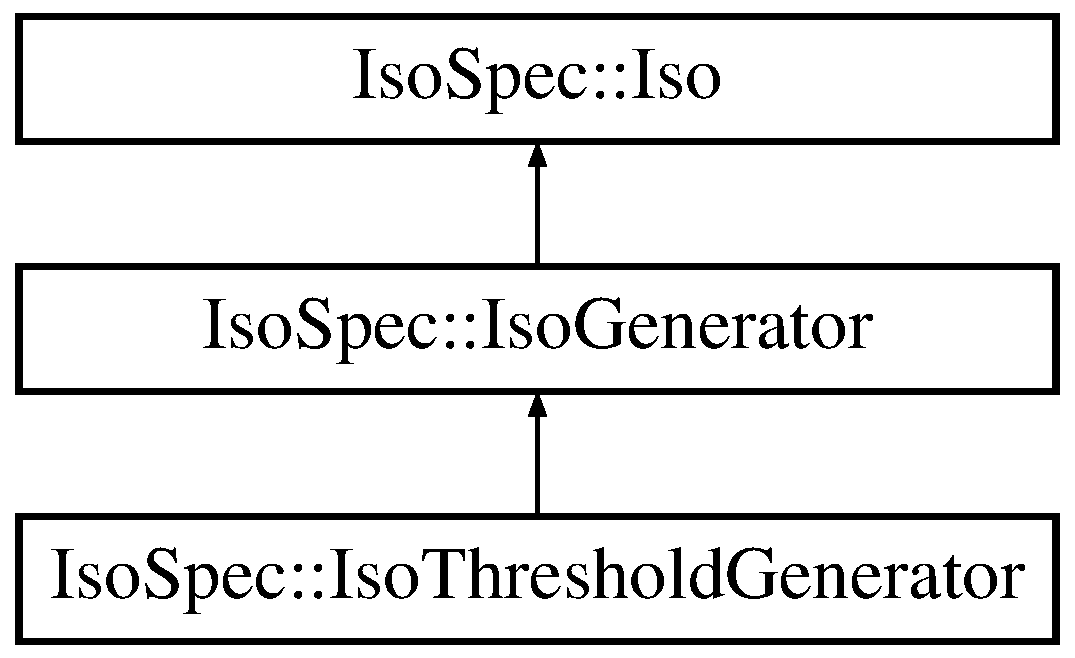
\includegraphics[height=3.000000cm]{class_iso_spec_1_1_iso_threshold_generator}
\end{center}
\end{figure}
\subsection*{Public Member Functions}
\begin{DoxyCompactItemize}
\item 
\mbox{\Hypertarget{class_iso_spec_1_1_iso_threshold_generator_a58699c4e68a846b979b8163bc6982e2c}\label{class_iso_spec_1_1_iso_threshold_generator_a58699c4e68a846b979b8163bc6982e2c}} 
void {\bfseries get\+\_\+conf\+\_\+signature} (int $\ast$space) const override final
\item 
\mbox{\hyperlink{class_iso_spec_1_1_iso_threshold_generator_a3abbcf1d810b6cad9400bd2552c3faf1}{Iso\+Threshold\+Generator}} (\mbox{\hyperlink{class_iso_spec_1_1_iso}{Iso}} \&\&iso, double \+\_\+threshold, bool \+\_\+absolute=true, int \+\_\+tab\+Size=1000, int \+\_\+hash\+Size=1000, bool reorder\+\_\+marginals=true)
\begin{DoxyCompactList}\small\item\em The move-\/constructor. \end{DoxyCompactList}\item 
I\+S\+O\+S\+P\+E\+C\+\_\+\+F\+O\+R\+C\+E\+\_\+\+I\+N\+L\+I\+NE bool \mbox{\hyperlink{class_iso_spec_1_1_iso_threshold_generator_a7164a6476b84665967c4a667a91d3f3e}{advance\+To\+Next\+Configuration}} () override final
\begin{DoxyCompactList}\small\item\em Advance to the next, not yet visited, most probable isotopologue. \end{DoxyCompactList}\item 
I\+S\+O\+S\+P\+E\+C\+\_\+\+F\+O\+R\+C\+E\+\_\+\+I\+N\+L\+I\+NE double \mbox{\hyperlink{class_iso_spec_1_1_iso_threshold_generator_a4aeebde03e385404d0175fd5696ff529}{lprob}} () const override final
\begin{DoxyCompactList}\small\item\em Get the log-\/probability of the current isotopologue. \end{DoxyCompactList}\item 
I\+S\+O\+S\+P\+E\+C\+\_\+\+F\+O\+R\+C\+E\+\_\+\+I\+N\+L\+I\+NE double \mbox{\hyperlink{class_iso_spec_1_1_iso_threshold_generator_ae2236accc7dc7a25a723e3c7317659b6}{mass}} () const override final
\begin{DoxyCompactList}\small\item\em Get the mass of the current isotopologue. \end{DoxyCompactList}\item 
I\+S\+O\+S\+P\+E\+C\+\_\+\+F\+O\+R\+C\+E\+\_\+\+I\+N\+L\+I\+NE double \mbox{\hyperlink{class_iso_spec_1_1_iso_threshold_generator_a998d987f81b2ca7ed610294f6a5f8df5}{prob}} () const override final
\begin{DoxyCompactList}\small\item\em Get the probability of the current isotopologue. \end{DoxyCompactList}\item 
\mbox{\Hypertarget{class_iso_spec_1_1_iso_threshold_generator_ac6aa2fff002a76b0beae1995f34ae5f6}\label{class_iso_spec_1_1_iso_threshold_generator_ac6aa2fff002a76b0beae1995f34ae5f6}} 
void \mbox{\hyperlink{class_iso_spec_1_1_iso_threshold_generator_ac6aa2fff002a76b0beae1995f34ae5f6}{terminate\+\_\+search}} ()
\begin{DoxyCompactList}\small\item\em Block the subsequent search of isotopologues. \end{DoxyCompactList}\item 
void \mbox{\hyperlink{class_iso_spec_1_1_iso_threshold_generator_ab830ffa21469df45a513ff1dcaf5d9e7}{reset}} ()
\item 
size\+\_\+t \mbox{\hyperlink{class_iso_spec_1_1_iso_threshold_generator_ad29d8761174bca7b1846ddec03b33528}{count\+\_\+confs}} ()
\end{DoxyCompactItemize}
\subsection*{Additional Inherited Members}


\subsection{Detailed Description}
The generator of isotopologues above a given threshold value. 

Attention\+: the calculated configurations are only partially ordeded and the user should not assume they will be ordered. This algorithm computes N isotopologues in O(\+N). It is a considerable advantage w.\+r.\+t. the \mbox{\hyperlink{class_iso_spec_1_1_iso_ordered_generator}{Iso\+Ordered\+Generator}}. 

Definition at line 235 of file iso\+Spec++.\+h.



\subsection{Constructor \& Destructor Documentation}
\mbox{\Hypertarget{class_iso_spec_1_1_iso_threshold_generator_a3abbcf1d810b6cad9400bd2552c3faf1}\label{class_iso_spec_1_1_iso_threshold_generator_a3abbcf1d810b6cad9400bd2552c3faf1}} 
\index{Iso\+Spec\+::\+Iso\+Threshold\+Generator@{Iso\+Spec\+::\+Iso\+Threshold\+Generator}!Iso\+Threshold\+Generator@{Iso\+Threshold\+Generator}}
\index{Iso\+Threshold\+Generator@{Iso\+Threshold\+Generator}!Iso\+Spec\+::\+Iso\+Threshold\+Generator@{Iso\+Spec\+::\+Iso\+Threshold\+Generator}}
\subsubsection{\texorpdfstring{Iso\+Threshold\+Generator()}{IsoThresholdGenerator()}}
{\footnotesize\ttfamily Iso\+Spec\+::\+Iso\+Threshold\+Generator\+::\+Iso\+Threshold\+Generator (\begin{DoxyParamCaption}\item[{\mbox{\hyperlink{class_iso_spec_1_1_iso}{Iso}} \&\&}]{iso,  }\item[{double}]{\+\_\+threshold,  }\item[{bool}]{\+\_\+absolute = {\ttfamily true},  }\item[{int}]{\+\_\+tab\+Size = {\ttfamily 1000},  }\item[{int}]{\+\_\+hash\+Size = {\ttfamily 1000},  }\item[{bool}]{reorder\+\_\+marginals = {\ttfamily true} }\end{DoxyParamCaption})}



The move-\/constructor. 


\begin{DoxyParams}{Parameters}
{\em iso} & An instance of the \mbox{\hyperlink{class_iso_spec_1_1_iso}{Iso}} class. \\
\hline
{\em \+\_\+threshold} & The threshold value. \\
\hline
{\em \+\_\+absolute} & If true, the \+\_\+threshold is interpreted as the absolute minimal peak height for the isotopologues. If false, the \+\_\+threshold is the fraction of the heighest peak\textquotesingle{}s probability. \\
\hline
{\em tab\+Size} & The size of the extension of the table with configurations. \\
\hline
{\em hash\+Size} & The size of the hash-\/table used to store subisotopologues and check if they have been already calculated. \\
\hline
\end{DoxyParams}


Definition at line 286 of file iso\+Spec++.\+cpp.



\subsection{Member Function Documentation}
\mbox{\Hypertarget{class_iso_spec_1_1_iso_threshold_generator_a7164a6476b84665967c4a667a91d3f3e}\label{class_iso_spec_1_1_iso_threshold_generator_a7164a6476b84665967c4a667a91d3f3e}} 
\index{Iso\+Spec\+::\+Iso\+Threshold\+Generator@{Iso\+Spec\+::\+Iso\+Threshold\+Generator}!advance\+To\+Next\+Configuration@{advance\+To\+Next\+Configuration}}
\index{advance\+To\+Next\+Configuration@{advance\+To\+Next\+Configuration}!Iso\+Spec\+::\+Iso\+Threshold\+Generator@{Iso\+Spec\+::\+Iso\+Threshold\+Generator}}
\subsubsection{\texorpdfstring{advance\+To\+Next\+Configuration()}{advanceToNextConfiguration()}}
{\footnotesize\ttfamily I\+S\+O\+S\+P\+E\+C\+\_\+\+F\+O\+R\+C\+E\+\_\+\+I\+N\+L\+I\+NE bool Iso\+Spec\+::\+Iso\+Threshold\+Generator\+::advance\+To\+Next\+Configuration (\begin{DoxyParamCaption}{ }\end{DoxyParamCaption})\hspace{0.3cm}{\ttfamily [inline]}, {\ttfamily [final]}, {\ttfamily [override]}, {\ttfamily [virtual]}}



Advance to the next, not yet visited, most probable isotopologue. 

\begin{DoxyReturn}{Returns}
Return false if it is not possible to advance. 
\end{DoxyReturn}


Implements \mbox{\hyperlink{class_iso_spec_1_1_iso_generator_a20f48ba18c6aecc57d73b2c3ec3a11dd}{Iso\+Spec\+::\+Iso\+Generator}}.



Definition at line 296 of file iso\+Spec++.\+h.

\mbox{\Hypertarget{class_iso_spec_1_1_iso_threshold_generator_ad29d8761174bca7b1846ddec03b33528}\label{class_iso_spec_1_1_iso_threshold_generator_ad29d8761174bca7b1846ddec03b33528}} 
\index{Iso\+Spec\+::\+Iso\+Threshold\+Generator@{Iso\+Spec\+::\+Iso\+Threshold\+Generator}!count\+\_\+confs@{count\+\_\+confs}}
\index{count\+\_\+confs@{count\+\_\+confs}!Iso\+Spec\+::\+Iso\+Threshold\+Generator@{Iso\+Spec\+::\+Iso\+Threshold\+Generator}}
\subsubsection{\texorpdfstring{count\+\_\+confs()}{count\_confs()}}
{\footnotesize\ttfamily size\+\_\+t Iso\+Spec\+::\+Iso\+Threshold\+Generator\+::count\+\_\+confs (\begin{DoxyParamCaption}{ }\end{DoxyParamCaption})}

Count the number of configurations in the distribution. This can be used to pre-\/allocate enough memory to store it (e.\+g. std\+::vector\textquotesingle{}s reserve() method -\/ this is faster than depending on the vector\textquotesingle{}s dynamic resizing, even though it means that the configuration space is walked through twice. This method has to be called before the first call to advance\+To\+Next\+Configuration and has undefined results (incl. segfaults) otherwise. 

Definition at line 376 of file iso\+Spec++.\+cpp.

\mbox{\Hypertarget{class_iso_spec_1_1_iso_threshold_generator_a4aeebde03e385404d0175fd5696ff529}\label{class_iso_spec_1_1_iso_threshold_generator_a4aeebde03e385404d0175fd5696ff529}} 
\index{Iso\+Spec\+::\+Iso\+Threshold\+Generator@{Iso\+Spec\+::\+Iso\+Threshold\+Generator}!lprob@{lprob}}
\index{lprob@{lprob}!Iso\+Spec\+::\+Iso\+Threshold\+Generator@{Iso\+Spec\+::\+Iso\+Threshold\+Generator}}
\subsubsection{\texorpdfstring{lprob()}{lprob()}}
{\footnotesize\ttfamily I\+S\+O\+S\+P\+E\+C\+\_\+\+F\+O\+R\+C\+E\+\_\+\+I\+N\+L\+I\+NE double Iso\+Spec\+::\+Iso\+Threshold\+Generator\+::lprob (\begin{DoxyParamCaption}{ }\end{DoxyParamCaption}) const\hspace{0.3cm}{\ttfamily [inline]}, {\ttfamily [final]}, {\ttfamily [override]}, {\ttfamily [virtual]}}



Get the log-\/probability of the current isotopologue. 

\begin{DoxyReturn}{Returns}
The log-\/probability of the current isotopologue. 
\end{DoxyReturn}


Reimplemented from \mbox{\hyperlink{class_iso_spec_1_1_iso_generator_ae8e24abbce51a4c93994f630acfdf383}{Iso\+Spec\+::\+Iso\+Generator}}.



Definition at line 335 of file iso\+Spec++.\+h.

\mbox{\Hypertarget{class_iso_spec_1_1_iso_threshold_generator_ae2236accc7dc7a25a723e3c7317659b6}\label{class_iso_spec_1_1_iso_threshold_generator_ae2236accc7dc7a25a723e3c7317659b6}} 
\index{Iso\+Spec\+::\+Iso\+Threshold\+Generator@{Iso\+Spec\+::\+Iso\+Threshold\+Generator}!mass@{mass}}
\index{mass@{mass}!Iso\+Spec\+::\+Iso\+Threshold\+Generator@{Iso\+Spec\+::\+Iso\+Threshold\+Generator}}
\subsubsection{\texorpdfstring{mass()}{mass()}}
{\footnotesize\ttfamily I\+S\+O\+S\+P\+E\+C\+\_\+\+F\+O\+R\+C\+E\+\_\+\+I\+N\+L\+I\+NE double Iso\+Spec\+::\+Iso\+Threshold\+Generator\+::mass (\begin{DoxyParamCaption}{ }\end{DoxyParamCaption}) const\hspace{0.3cm}{\ttfamily [inline]}, {\ttfamily [final]}, {\ttfamily [override]}, {\ttfamily [virtual]}}



Get the mass of the current isotopologue. 

\begin{DoxyReturn}{Returns}
The mass of the current isotopologue. 
\end{DoxyReturn}


Reimplemented from \mbox{\hyperlink{class_iso_spec_1_1_iso_generator_a34173228ef73e272e2ff0ae6ce58092d}{Iso\+Spec\+::\+Iso\+Generator}}.



Definition at line 336 of file iso\+Spec++.\+h.

\mbox{\Hypertarget{class_iso_spec_1_1_iso_threshold_generator_a998d987f81b2ca7ed610294f6a5f8df5}\label{class_iso_spec_1_1_iso_threshold_generator_a998d987f81b2ca7ed610294f6a5f8df5}} 
\index{Iso\+Spec\+::\+Iso\+Threshold\+Generator@{Iso\+Spec\+::\+Iso\+Threshold\+Generator}!prob@{prob}}
\index{prob@{prob}!Iso\+Spec\+::\+Iso\+Threshold\+Generator@{Iso\+Spec\+::\+Iso\+Threshold\+Generator}}
\subsubsection{\texorpdfstring{prob()}{prob()}}
{\footnotesize\ttfamily I\+S\+O\+S\+P\+E\+C\+\_\+\+F\+O\+R\+C\+E\+\_\+\+I\+N\+L\+I\+NE double Iso\+Spec\+::\+Iso\+Threshold\+Generator\+::prob (\begin{DoxyParamCaption}{ }\end{DoxyParamCaption}) const\hspace{0.3cm}{\ttfamily [inline]}, {\ttfamily [final]}, {\ttfamily [override]}, {\ttfamily [virtual]}}



Get the probability of the current isotopologue. 

\begin{DoxyReturn}{Returns}
The probability of the current isotopologue. 
\end{DoxyReturn}


Reimplemented from \mbox{\hyperlink{class_iso_spec_1_1_iso_generator_aecf1b3292fcc0857a86efe619a37fff0}{Iso\+Spec\+::\+Iso\+Generator}}.



Definition at line 337 of file iso\+Spec++.\+h.

\mbox{\Hypertarget{class_iso_spec_1_1_iso_threshold_generator_ab830ffa21469df45a513ff1dcaf5d9e7}\label{class_iso_spec_1_1_iso_threshold_generator_ab830ffa21469df45a513ff1dcaf5d9e7}} 
\index{Iso\+Spec\+::\+Iso\+Threshold\+Generator@{Iso\+Spec\+::\+Iso\+Threshold\+Generator}!reset@{reset}}
\index{reset@{reset}!Iso\+Spec\+::\+Iso\+Threshold\+Generator@{Iso\+Spec\+::\+Iso\+Threshold\+Generator}}
\subsubsection{\texorpdfstring{reset()}{reset()}}
{\footnotesize\ttfamily void Iso\+Spec\+::\+Iso\+Threshold\+Generator\+::reset (\begin{DoxyParamCaption}{ }\end{DoxyParamCaption})}

Reset the generator to the beginning of the sequence. Allows it to be reused, eg. to go through the conf space once, calculate the amount of space needed to store configurations, then to allocate that memory, and go through it again, this time saving configurations (and {\itshape is} in fact faster than allocating a std\+::vector and depending on it to grow as needed. This is cheaper than throwing away the generator and making a new one too\+: marginal distributions don\textquotesingle{}t need to be recalculated. 

Definition at line 386 of file iso\+Spec++.\+cpp.



The documentation for this class was generated from the following files\+:\begin{DoxyCompactItemize}
\item 
/\+Users/matteo/\+Projects/isospec/\+Iso\+Spec/\+Iso\+Spec++/iso\+Spec++.\+h\item 
/\+Users/matteo/\+Projects/isospec/\+Iso\+Spec/\+Iso\+Spec++/iso\+Spec++.\+cpp\end{DoxyCompactItemize}

\hypertarget{class_iso_spec_1_1_key_hasher}{}\section{Iso\+Spec\+:\+:Key\+Hasher Class Reference}
\label{class_iso_spec_1_1_key_hasher}\index{Iso\+Spec\+::\+Key\+Hasher@{Iso\+Spec\+::\+Key\+Hasher}}
\subsection*{Public Member Functions}
\begin{DoxyCompactItemize}
\item 
\mbox{\Hypertarget{class_iso_spec_1_1_key_hasher_a094e6c2b6a3c9fa09b81187cbdf50de3}\label{class_iso_spec_1_1_key_hasher_a094e6c2b6a3c9fa09b81187cbdf50de3}} 
{\bfseries Key\+Hasher} (int dim)
\item 
\mbox{\Hypertarget{class_iso_spec_1_1_key_hasher_a32c10222b6c45a5f0f290821c476e83f}\label{class_iso_spec_1_1_key_hasher_a32c10222b6c45a5f0f290821c476e83f}} 
std\+::size\+\_\+t {\bfseries operator()} (const int $\ast$conf) const
\end{DoxyCompactItemize}


\subsection{Detailed Description}


Definition at line 27 of file operators.\+h.



The documentation for this class was generated from the following files\+:\begin{DoxyCompactItemize}
\item 
/\+Users/matteo/\+Projects/isospec/\+Iso\+Spec/\+Iso\+Spec++/operators.\+h\item 
/\+Users/matteo/\+Projects/isospec/\+Iso\+Spec/\+Iso\+Spec++/operators.\+cpp\end{DoxyCompactItemize}

\hypertarget{class_iso_spec_1_1_marginal}{}\section{Iso\+Spec\+:\+:Marginal Class Reference}
\label{class_iso_spec_1_1_marginal}\index{Iso\+Spec\+::\+Marginal@{Iso\+Spec\+::\+Marginal}}


The marginal distribution class (a subisotopologue).  




{\ttfamily \#include $<$marginal\+Trek++.\+h$>$}

Inheritance diagram for Iso\+Spec\+:\+:Marginal\+:\begin{figure}[H]
\begin{center}
\leavevmode
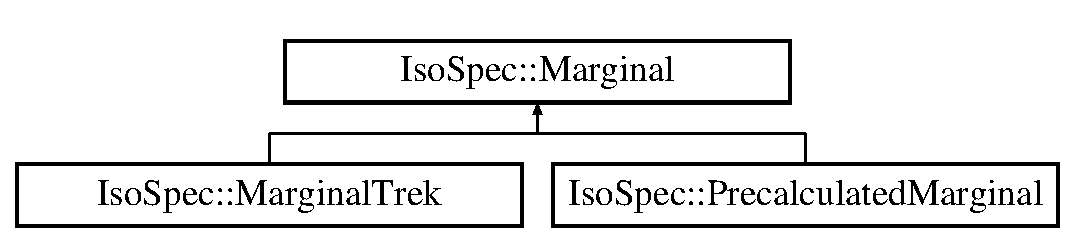
\includegraphics[height=2.000000cm]{class_iso_spec_1_1_marginal}
\end{center}
\end{figure}
\subsection*{Public Member Functions}
\begin{DoxyCompactItemize}
\item 
\mbox{\hyperlink{class_iso_spec_1_1_marginal_a46be0c1cf5b169a54056997ba404183c}{Marginal}} (const double $\ast$\+\_\+masses, const double $\ast$\+\_\+probs, int \+\_\+isotope\+No, int \+\_\+atom\+Cnt)
\begin{DoxyCompactList}\small\item\em Class constructor. \end{DoxyCompactList}\item 
\mbox{\Hypertarget{class_iso_spec_1_1_marginal_a02e8f92f8f9add352840f5dba8de5e06}\label{class_iso_spec_1_1_marginal_a02e8f92f8f9add352840f5dba8de5e06}} 
{\bfseries Marginal} (\mbox{\hyperlink{class_iso_spec_1_1_marginal}{Marginal}} \&other)=delete
\item 
\mbox{\Hypertarget{class_iso_spec_1_1_marginal_a9120cad240058afc3705951d80d28a10}\label{class_iso_spec_1_1_marginal_a9120cad240058afc3705951d80d28a10}} 
\mbox{\hyperlink{class_iso_spec_1_1_marginal}{Marginal}} \& {\bfseries operator=} (const \mbox{\hyperlink{class_iso_spec_1_1_marginal}{Marginal}} \&other)=delete
\item 
\mbox{\Hypertarget{class_iso_spec_1_1_marginal_ad60fff17fa2c68ea2cd7f183a635379e}\label{class_iso_spec_1_1_marginal_ad60fff17fa2c68ea2cd7f183a635379e}} 
\mbox{\hyperlink{class_iso_spec_1_1_marginal_ad60fff17fa2c68ea2cd7f183a635379e}{Marginal}} (\mbox{\hyperlink{class_iso_spec_1_1_marginal}{Marginal}} \&\&other)
\begin{DoxyCompactList}\small\item\em Move constructor. \end{DoxyCompactList}\item 
\mbox{\Hypertarget{class_iso_spec_1_1_marginal_ad44004fa1e83c4a53d431ca403ce3ae4}\label{class_iso_spec_1_1_marginal_ad44004fa1e83c4a53d431ca403ce3ae4}} 
virtual \mbox{\hyperlink{class_iso_spec_1_1_marginal_ad44004fa1e83c4a53d431ca403ce3ae4}{$\sim$\+Marginal}} ()
\begin{DoxyCompactList}\small\item\em Destructor. \end{DoxyCompactList}\item 
int \mbox{\hyperlink{class_iso_spec_1_1_marginal_a05aa80c3fa77a0406102731934db1a83}{get\+\_\+isotope\+No}} () const
\begin{DoxyCompactList}\small\item\em Get the number of isotopes of the investigated element. \end{DoxyCompactList}\item 
double \mbox{\hyperlink{class_iso_spec_1_1_marginal_a8b67c507263973da53e533d804e23ac9}{get\+Lightest\+Conf\+Mass}} () const
\begin{DoxyCompactList}\small\item\em Get the mass of the lightest subisotopologue. \end{DoxyCompactList}\item 
double \mbox{\hyperlink{class_iso_spec_1_1_marginal_aa5598b4d2b31b5daec1c2bac653d0aff}{get\+Heaviest\+Conf\+Mass}} () const
\begin{DoxyCompactList}\small\item\em Get the mass of the heaviest subisotopologue. \end{DoxyCompactList}\item 
double \mbox{\hyperlink{class_iso_spec_1_1_marginal_ac9408957145d2aa63af32f6647c8ea49}{get\+Mode\+L\+Prob}} () const
\begin{DoxyCompactList}\small\item\em Get the log-\/probability of the mode subisotopologue. \end{DoxyCompactList}\item 
double \mbox{\hyperlink{class_iso_spec_1_1_marginal_ad2121802133075a87f0987dc27d0617f}{get\+Mode\+Mass}} () const
\begin{DoxyCompactList}\small\item\em The the mass of the mode subisotopologue. \end{DoxyCompactList}\item 
double \mbox{\hyperlink{class_iso_spec_1_1_marginal_a7bc1eeba342977de3a77c3c7e6ca55b0}{get\+Mode\+Prob}} () const
\begin{DoxyCompactList}\small\item\em The the probability of the mode subisotopologue. \end{DoxyCompactList}\item 
double \mbox{\hyperlink{class_iso_spec_1_1_marginal_a3f9607f51efcfdac1ca58a1467e3a5dc}{get\+Smallest\+L\+Prob}} () const
\begin{DoxyCompactList}\small\item\em The the log-\/probability of the lightest subisotopologue. \end{DoxyCompactList}\item 
double \mbox{\hyperlink{class_iso_spec_1_1_marginal_a1974bb030ce70178da569214b4b93cb8}{log\+Prob}} (Conf conf) const
\begin{DoxyCompactList}\small\item\em Calculate the log-\/probability of a given subisotopologue. \end{DoxyCompactList}\end{DoxyCompactItemize}
\subsection*{Protected Attributes}
\begin{DoxyCompactItemize}
\item 
const unsigned int \mbox{\hyperlink{class_iso_spec_1_1_marginal_a8dd6415882661f7b9ceedbe09bc200e3}{isotope\+No}}
\item 
const unsigned int \mbox{\hyperlink{class_iso_spec_1_1_marginal_a53c2af7dcb84aa9d5e0e0918fe7875cd}{atom\+Cnt}}
\item 
const double $\ast$const \mbox{\hyperlink{class_iso_spec_1_1_marginal_a91265e07f5bb65314995f816f5a9c729}{atom\+\_\+masses}}
\item 
const double $\ast$const \mbox{\hyperlink{class_iso_spec_1_1_marginal_af059df011e707781fdd4c1d7b70bd91a}{atom\+\_\+l\+Probs}}
\item 
const double \mbox{\hyperlink{class_iso_spec_1_1_marginal_aa3fb5ed3a9b63a855d6270287aed7417}{loggamma\+\_\+nominator}}
\item 
const Conf \mbox{\hyperlink{class_iso_spec_1_1_marginal_a640f3b44605b510ee556a25e35a2e095}{mode\+\_\+conf}}
\item 
const double \mbox{\hyperlink{class_iso_spec_1_1_marginal_a38238e7581f59f08d0faf8ab5eabc0dc}{mode\+\_\+lprob}}
\item 
const double \mbox{\hyperlink{class_iso_spec_1_1_marginal_a3bfea931e5e1ec1e7d90e8e096c38eb7}{mode\+\_\+mass}}
\item 
const double \mbox{\hyperlink{class_iso_spec_1_1_marginal_a75315ec4c470be5f82b903172f7c43ae}{mode\+\_\+prob}}
\item 
const double \mbox{\hyperlink{class_iso_spec_1_1_marginal_a2abd05ba9351e21cd99e2783e26bd6dc}{smallest\+\_\+lprob}}
\end{DoxyCompactItemize}


\subsection{Detailed Description}
The marginal distribution class (a subisotopologue). 

This class mostly provides some basic common A\+PI for subclasses, but itself is not abstract. This class represents the probability distribution generated by one element only -- a subisotopologue. For instance, it might be the distribution of C200, that might be part of, say, C200\+H402. It corresponds to the multinomial distribution, where each configuration can also be attributed a precise mass. The constructor method perform initial hill-\/climbing to find the most probable sub-\/isotopologue (the mode). 

Definition at line 45 of file marginal\+Trek++.\+h.



\subsection{Constructor \& Destructor Documentation}
\mbox{\Hypertarget{class_iso_spec_1_1_marginal_a46be0c1cf5b169a54056997ba404183c}\label{class_iso_spec_1_1_marginal_a46be0c1cf5b169a54056997ba404183c}} 
\index{Iso\+Spec\+::\+Marginal@{Iso\+Spec\+::\+Marginal}!Marginal@{Marginal}}
\index{Marginal@{Marginal}!Iso\+Spec\+::\+Marginal@{Iso\+Spec\+::\+Marginal}}
\subsubsection{\texorpdfstring{Marginal()}{Marginal()}}
{\footnotesize\ttfamily Iso\+Spec\+::\+Marginal\+::\+Marginal (\begin{DoxyParamCaption}\item[{const double $\ast$}]{\+\_\+masses,  }\item[{const double $\ast$}]{\+\_\+probs,  }\item[{int}]{\+\_\+isotope\+No,  }\item[{int}]{\+\_\+atom\+Cnt }\end{DoxyParamCaption})}



Class constructor. 


\begin{DoxyParams}{Parameters}
{\em \+\_\+masses} & A table of masses of the stable isotopes of the investigated element, e.\+g. for C10 it is 2\+: C12 and C13. \\
\hline
{\em \+\_\+probs} & A table of natural frequencies of the stable isotopes of the investigated element, see I\+U\+P\+AC at \href{https://iupac.org/isotopesmatter/}{\tt https\+://iupac.\+org/isotopesmatter/} \\
\hline
{\em \+\_\+isotope\+No} & Number of isotopes of a given element. \\
\hline
{\em \+\_\+atom\+Cnt} & The number of atoms of the given element, e.\+g. 10 for C10. \\
\hline
\end{DoxyParams}
\begin{DoxyReturn}{Returns}
An instance of the \mbox{\hyperlink{class_iso_spec_1_1_marginal}{Marginal}} class. 
\end{DoxyReturn}


Definition at line 187 of file marginal\+Trek++.\+cpp.



\subsection{Member Function Documentation}
\mbox{\Hypertarget{class_iso_spec_1_1_marginal_a05aa80c3fa77a0406102731934db1a83}\label{class_iso_spec_1_1_marginal_a05aa80c3fa77a0406102731934db1a83}} 
\index{Iso\+Spec\+::\+Marginal@{Iso\+Spec\+::\+Marginal}!get\+\_\+isotope\+No@{get\+\_\+isotope\+No}}
\index{get\+\_\+isotope\+No@{get\+\_\+isotope\+No}!Iso\+Spec\+::\+Marginal@{Iso\+Spec\+::\+Marginal}}
\subsubsection{\texorpdfstring{get\+\_\+isotope\+No()}{get\_isotopeNo()}}
{\footnotesize\ttfamily int Iso\+Spec\+::\+Marginal\+::get\+\_\+isotope\+No (\begin{DoxyParamCaption}{ }\end{DoxyParamCaption}) const\hspace{0.3cm}{\ttfamily [inline]}}



Get the number of isotopes of the investigated element. 

\begin{DoxyReturn}{Returns}
The integer number of isotopes of the investigated element. 
\end{DoxyReturn}


Definition at line 92 of file marginal\+Trek++.\+h.

\mbox{\Hypertarget{class_iso_spec_1_1_marginal_aa5598b4d2b31b5daec1c2bac653d0aff}\label{class_iso_spec_1_1_marginal_aa5598b4d2b31b5daec1c2bac653d0aff}} 
\index{Iso\+Spec\+::\+Marginal@{Iso\+Spec\+::\+Marginal}!get\+Heaviest\+Conf\+Mass@{get\+Heaviest\+Conf\+Mass}}
\index{get\+Heaviest\+Conf\+Mass@{get\+Heaviest\+Conf\+Mass}!Iso\+Spec\+::\+Marginal@{Iso\+Spec\+::\+Marginal}}
\subsubsection{\texorpdfstring{get\+Heaviest\+Conf\+Mass()}{getHeaviestConfMass()}}
{\footnotesize\ttfamily double Iso\+Spec\+::\+Marginal\+::get\+Heaviest\+Conf\+Mass (\begin{DoxyParamCaption}{ }\end{DoxyParamCaption}) const}



Get the mass of the heaviest subisotopologue. 

This is trivially obtained by considering all atom\+No atoms to be the heaviest isotope possible. \begin{DoxyReturn}{Returns}
The mass of the heaviest subisotopologue. 
\end{DoxyReturn}


Definition at line 246 of file marginal\+Trek++.\+cpp.

\mbox{\Hypertarget{class_iso_spec_1_1_marginal_a8b67c507263973da53e533d804e23ac9}\label{class_iso_spec_1_1_marginal_a8b67c507263973da53e533d804e23ac9}} 
\index{Iso\+Spec\+::\+Marginal@{Iso\+Spec\+::\+Marginal}!get\+Lightest\+Conf\+Mass@{get\+Lightest\+Conf\+Mass}}
\index{get\+Lightest\+Conf\+Mass@{get\+Lightest\+Conf\+Mass}!Iso\+Spec\+::\+Marginal@{Iso\+Spec\+::\+Marginal}}
\subsubsection{\texorpdfstring{get\+Lightest\+Conf\+Mass()}{getLightestConfMass()}}
{\footnotesize\ttfamily double Iso\+Spec\+::\+Marginal\+::get\+Lightest\+Conf\+Mass (\begin{DoxyParamCaption}{ }\end{DoxyParamCaption}) const}



Get the mass of the lightest subisotopologue. 

This is trivially obtained by considering all atom\+No atoms to be the lightest isotope possible. \begin{DoxyReturn}{Returns}
The mass of the lightiest subisotopologue. 
\end{DoxyReturn}


Definition at line 237 of file marginal\+Trek++.\+cpp.

\mbox{\Hypertarget{class_iso_spec_1_1_marginal_ac9408957145d2aa63af32f6647c8ea49}\label{class_iso_spec_1_1_marginal_ac9408957145d2aa63af32f6647c8ea49}} 
\index{Iso\+Spec\+::\+Marginal@{Iso\+Spec\+::\+Marginal}!get\+Mode\+L\+Prob@{get\+Mode\+L\+Prob}}
\index{get\+Mode\+L\+Prob@{get\+Mode\+L\+Prob}!Iso\+Spec\+::\+Marginal@{Iso\+Spec\+::\+Marginal}}
\subsubsection{\texorpdfstring{get\+Mode\+L\+Prob()}{getModeLProb()}}
{\footnotesize\ttfamily double Iso\+Spec\+::\+Marginal\+::get\+Mode\+L\+Prob (\begin{DoxyParamCaption}{ }\end{DoxyParamCaption}) const\hspace{0.3cm}{\ttfamily [inline]}}



Get the log-\/probability of the mode subisotopologue. 

\begin{DoxyReturn}{Returns}
The log-\/probability of a/the most probable subisotopologue. 
\end{DoxyReturn}


Definition at line 110 of file marginal\+Trek++.\+h.

\mbox{\Hypertarget{class_iso_spec_1_1_marginal_ad2121802133075a87f0987dc27d0617f}\label{class_iso_spec_1_1_marginal_ad2121802133075a87f0987dc27d0617f}} 
\index{Iso\+Spec\+::\+Marginal@{Iso\+Spec\+::\+Marginal}!get\+Mode\+Mass@{get\+Mode\+Mass}}
\index{get\+Mode\+Mass@{get\+Mode\+Mass}!Iso\+Spec\+::\+Marginal@{Iso\+Spec\+::\+Marginal}}
\subsubsection{\texorpdfstring{get\+Mode\+Mass()}{getModeMass()}}
{\footnotesize\ttfamily double Iso\+Spec\+::\+Marginal\+::get\+Mode\+Mass (\begin{DoxyParamCaption}{ }\end{DoxyParamCaption}) const\hspace{0.3cm}{\ttfamily [inline]}}



The the mass of the mode subisotopologue. 

\begin{DoxyReturn}{Returns}
The mass of one of the most probable subisotopologues. 
\end{DoxyReturn}


Definition at line 116 of file marginal\+Trek++.\+h.

\mbox{\Hypertarget{class_iso_spec_1_1_marginal_a7bc1eeba342977de3a77c3c7e6ca55b0}\label{class_iso_spec_1_1_marginal_a7bc1eeba342977de3a77c3c7e6ca55b0}} 
\index{Iso\+Spec\+::\+Marginal@{Iso\+Spec\+::\+Marginal}!get\+Mode\+Prob@{get\+Mode\+Prob}}
\index{get\+Mode\+Prob@{get\+Mode\+Prob}!Iso\+Spec\+::\+Marginal@{Iso\+Spec\+::\+Marginal}}
\subsubsection{\texorpdfstring{get\+Mode\+Prob()}{getModeProb()}}
{\footnotesize\ttfamily double Iso\+Spec\+::\+Marginal\+::get\+Mode\+Prob (\begin{DoxyParamCaption}{ }\end{DoxyParamCaption}) const\hspace{0.3cm}{\ttfamily [inline]}}



The the probability of the mode subisotopologue. 

\begin{DoxyReturn}{Returns}
The probability of a/the most probable subisotopologue. 
\end{DoxyReturn}


Definition at line 122 of file marginal\+Trek++.\+h.

\mbox{\Hypertarget{class_iso_spec_1_1_marginal_a3f9607f51efcfdac1ca58a1467e3a5dc}\label{class_iso_spec_1_1_marginal_a3f9607f51efcfdac1ca58a1467e3a5dc}} 
\index{Iso\+Spec\+::\+Marginal@{Iso\+Spec\+::\+Marginal}!get\+Smallest\+L\+Prob@{get\+Smallest\+L\+Prob}}
\index{get\+Smallest\+L\+Prob@{get\+Smallest\+L\+Prob}!Iso\+Spec\+::\+Marginal@{Iso\+Spec\+::\+Marginal}}
\subsubsection{\texorpdfstring{get\+Smallest\+L\+Prob()}{getSmallestLProb()}}
{\footnotesize\ttfamily double Iso\+Spec\+::\+Marginal\+::get\+Smallest\+L\+Prob (\begin{DoxyParamCaption}{ }\end{DoxyParamCaption}) const\hspace{0.3cm}{\ttfamily [inline]}}



The the log-\/probability of the lightest subisotopologue. 

\begin{DoxyReturn}{Returns}
The logarithm of the smallest non-\/zero probability of a subisotopologue. 
\end{DoxyReturn}


Definition at line 129 of file marginal\+Trek++.\+h.

\mbox{\Hypertarget{class_iso_spec_1_1_marginal_a1974bb030ce70178da569214b4b93cb8}\label{class_iso_spec_1_1_marginal_a1974bb030ce70178da569214b4b93cb8}} 
\index{Iso\+Spec\+::\+Marginal@{Iso\+Spec\+::\+Marginal}!log\+Prob@{log\+Prob}}
\index{log\+Prob@{log\+Prob}!Iso\+Spec\+::\+Marginal@{Iso\+Spec\+::\+Marginal}}
\subsubsection{\texorpdfstring{log\+Prob()}{logProb()}}
{\footnotesize\ttfamily double Iso\+Spec\+::\+Marginal\+::log\+Prob (\begin{DoxyParamCaption}\item[{Conf}]{conf }\end{DoxyParamCaption}) const\hspace{0.3cm}{\ttfamily [inline]}}



Calculate the log-\/probability of a given subisotopologue. 


\begin{DoxyParams}{Parameters}
{\em conf} & A subisotopologue (a table of integers describing subsequent isotope-\/counts). \\
\hline
\end{DoxyParams}
\begin{DoxyReturn}{Returns}
The log-\/probability of the input subisotopologue. 
\end{DoxyReturn}


Definition at line 136 of file marginal\+Trek++.\+h.



\subsection{Member Data Documentation}
\mbox{\Hypertarget{class_iso_spec_1_1_marginal_af059df011e707781fdd4c1d7b70bd91a}\label{class_iso_spec_1_1_marginal_af059df011e707781fdd4c1d7b70bd91a}} 
\index{Iso\+Spec\+::\+Marginal@{Iso\+Spec\+::\+Marginal}!atom\+\_\+l\+Probs@{atom\+\_\+l\+Probs}}
\index{atom\+\_\+l\+Probs@{atom\+\_\+l\+Probs}!Iso\+Spec\+::\+Marginal@{Iso\+Spec\+::\+Marginal}}
\subsubsection{\texorpdfstring{atom\+\_\+l\+Probs}{atom\_lProbs}}
{\footnotesize\ttfamily const double$\ast$ const Iso\+Spec\+::\+Marginal\+::atom\+\_\+l\+Probs\hspace{0.3cm}{\ttfamily [protected]}}

Table of log-\/probabilities of all the isotope\+No isotopes. 

Definition at line 53 of file marginal\+Trek++.\+h.

\mbox{\Hypertarget{class_iso_spec_1_1_marginal_a91265e07f5bb65314995f816f5a9c729}\label{class_iso_spec_1_1_marginal_a91265e07f5bb65314995f816f5a9c729}} 
\index{Iso\+Spec\+::\+Marginal@{Iso\+Spec\+::\+Marginal}!atom\+\_\+masses@{atom\+\_\+masses}}
\index{atom\+\_\+masses@{atom\+\_\+masses}!Iso\+Spec\+::\+Marginal@{Iso\+Spec\+::\+Marginal}}
\subsubsection{\texorpdfstring{atom\+\_\+masses}{atom\_masses}}
{\footnotesize\ttfamily const double$\ast$ const Iso\+Spec\+::\+Marginal\+::atom\+\_\+masses\hspace{0.3cm}{\ttfamily [protected]}}

Table of atomic masses of all the isotope\+No isotopes. 

Definition at line 52 of file marginal\+Trek++.\+h.

\mbox{\Hypertarget{class_iso_spec_1_1_marginal_a53c2af7dcb84aa9d5e0e0918fe7875cd}\label{class_iso_spec_1_1_marginal_a53c2af7dcb84aa9d5e0e0918fe7875cd}} 
\index{Iso\+Spec\+::\+Marginal@{Iso\+Spec\+::\+Marginal}!atom\+Cnt@{atom\+Cnt}}
\index{atom\+Cnt@{atom\+Cnt}!Iso\+Spec\+::\+Marginal@{Iso\+Spec\+::\+Marginal}}
\subsubsection{\texorpdfstring{atom\+Cnt}{atomCnt}}
{\footnotesize\ttfamily const unsigned int Iso\+Spec\+::\+Marginal\+::atom\+Cnt\hspace{0.3cm}{\ttfamily [protected]}}

The number of atoms of the given element. 

Definition at line 51 of file marginal\+Trek++.\+h.

\mbox{\Hypertarget{class_iso_spec_1_1_marginal_a8dd6415882661f7b9ceedbe09bc200e3}\label{class_iso_spec_1_1_marginal_a8dd6415882661f7b9ceedbe09bc200e3}} 
\index{Iso\+Spec\+::\+Marginal@{Iso\+Spec\+::\+Marginal}!isotope\+No@{isotope\+No}}
\index{isotope\+No@{isotope\+No}!Iso\+Spec\+::\+Marginal@{Iso\+Spec\+::\+Marginal}}
\subsubsection{\texorpdfstring{isotope\+No}{isotopeNo}}
{\footnotesize\ttfamily const unsigned int Iso\+Spec\+::\+Marginal\+::isotope\+No\hspace{0.3cm}{\ttfamily [protected]}}

The number of isotopes of the given element. 

Definition at line 50 of file marginal\+Trek++.\+h.

\mbox{\Hypertarget{class_iso_spec_1_1_marginal_aa3fb5ed3a9b63a855d6270287aed7417}\label{class_iso_spec_1_1_marginal_aa3fb5ed3a9b63a855d6270287aed7417}} 
\index{Iso\+Spec\+::\+Marginal@{Iso\+Spec\+::\+Marginal}!loggamma\+\_\+nominator@{loggamma\+\_\+nominator}}
\index{loggamma\+\_\+nominator@{loggamma\+\_\+nominator}!Iso\+Spec\+::\+Marginal@{Iso\+Spec\+::\+Marginal}}
\subsubsection{\texorpdfstring{loggamma\+\_\+nominator}{loggamma\_nominator}}
{\footnotesize\ttfamily const double Iso\+Spec\+::\+Marginal\+::loggamma\+\_\+nominator\hspace{0.3cm}{\ttfamily [protected]}}

The constant nominator that appears in the expressions for the multinomial probabilities. 

Definition at line 54 of file marginal\+Trek++.\+h.

\mbox{\Hypertarget{class_iso_spec_1_1_marginal_a640f3b44605b510ee556a25e35a2e095}\label{class_iso_spec_1_1_marginal_a640f3b44605b510ee556a25e35a2e095}} 
\index{Iso\+Spec\+::\+Marginal@{Iso\+Spec\+::\+Marginal}!mode\+\_\+conf@{mode\+\_\+conf}}
\index{mode\+\_\+conf@{mode\+\_\+conf}!Iso\+Spec\+::\+Marginal@{Iso\+Spec\+::\+Marginal}}
\subsubsection{\texorpdfstring{mode\+\_\+conf}{mode\_conf}}
{\footnotesize\ttfamily const Conf Iso\+Spec\+::\+Marginal\+::mode\+\_\+conf\hspace{0.3cm}{\ttfamily [protected]}}

A subisotopologue with most probability. If not unique, one of the representatives of that class of subisotopologues. 

Definition at line 55 of file marginal\+Trek++.\+h.

\mbox{\Hypertarget{class_iso_spec_1_1_marginal_a38238e7581f59f08d0faf8ab5eabc0dc}\label{class_iso_spec_1_1_marginal_a38238e7581f59f08d0faf8ab5eabc0dc}} 
\index{Iso\+Spec\+::\+Marginal@{Iso\+Spec\+::\+Marginal}!mode\+\_\+lprob@{mode\+\_\+lprob}}
\index{mode\+\_\+lprob@{mode\+\_\+lprob}!Iso\+Spec\+::\+Marginal@{Iso\+Spec\+::\+Marginal}}
\subsubsection{\texorpdfstring{mode\+\_\+lprob}{mode\_lprob}}
{\footnotesize\ttfamily const double Iso\+Spec\+::\+Marginal\+::mode\+\_\+lprob\hspace{0.3cm}{\ttfamily [protected]}}

The log-\/probability of the mode subisotopologue. 

Definition at line 56 of file marginal\+Trek++.\+h.

\mbox{\Hypertarget{class_iso_spec_1_1_marginal_a3bfea931e5e1ec1e7d90e8e096c38eb7}\label{class_iso_spec_1_1_marginal_a3bfea931e5e1ec1e7d90e8e096c38eb7}} 
\index{Iso\+Spec\+::\+Marginal@{Iso\+Spec\+::\+Marginal}!mode\+\_\+mass@{mode\+\_\+mass}}
\index{mode\+\_\+mass@{mode\+\_\+mass}!Iso\+Spec\+::\+Marginal@{Iso\+Spec\+::\+Marginal}}
\subsubsection{\texorpdfstring{mode\+\_\+mass}{mode\_mass}}
{\footnotesize\ttfamily const double Iso\+Spec\+::\+Marginal\+::mode\+\_\+mass\hspace{0.3cm}{\ttfamily [protected]}}

The mass of the mode subisotopologue. 

Definition at line 57 of file marginal\+Trek++.\+h.

\mbox{\Hypertarget{class_iso_spec_1_1_marginal_a75315ec4c470be5f82b903172f7c43ae}\label{class_iso_spec_1_1_marginal_a75315ec4c470be5f82b903172f7c43ae}} 
\index{Iso\+Spec\+::\+Marginal@{Iso\+Spec\+::\+Marginal}!mode\+\_\+prob@{mode\+\_\+prob}}
\index{mode\+\_\+prob@{mode\+\_\+prob}!Iso\+Spec\+::\+Marginal@{Iso\+Spec\+::\+Marginal}}
\subsubsection{\texorpdfstring{mode\+\_\+prob}{mode\_prob}}
{\footnotesize\ttfamily const double Iso\+Spec\+::\+Marginal\+::mode\+\_\+prob\hspace{0.3cm}{\ttfamily [protected]}}

The probability of the mode subisotopologue. 

Definition at line 58 of file marginal\+Trek++.\+h.

\mbox{\Hypertarget{class_iso_spec_1_1_marginal_a2abd05ba9351e21cd99e2783e26bd6dc}\label{class_iso_spec_1_1_marginal_a2abd05ba9351e21cd99e2783e26bd6dc}} 
\index{Iso\+Spec\+::\+Marginal@{Iso\+Spec\+::\+Marginal}!smallest\+\_\+lprob@{smallest\+\_\+lprob}}
\index{smallest\+\_\+lprob@{smallest\+\_\+lprob}!Iso\+Spec\+::\+Marginal@{Iso\+Spec\+::\+Marginal}}
\subsubsection{\texorpdfstring{smallest\+\_\+lprob}{smallest\_lprob}}
{\footnotesize\ttfamily const double Iso\+Spec\+::\+Marginal\+::smallest\+\_\+lprob\hspace{0.3cm}{\ttfamily [protected]}}

The smallest-\/achievable log-\/probability in the distribution of subisotopologues. 

Definition at line 59 of file marginal\+Trek++.\+h.



The documentation for this class was generated from the following files\+:\begin{DoxyCompactItemize}
\item 
/\+Users/matteo/\+Projects/isospec/\+Iso\+Spec/\+Iso\+Spec++/marginal\+Trek++.\+h\item 
/\+Users/matteo/\+Projects/isospec/\+Iso\+Spec/\+Iso\+Spec++/marginal\+Trek++.\+cpp\end{DoxyCompactItemize}

\hypertarget{class_iso_spec_1_1_marginal_trek}{}\section{Iso\+Spec\+:\+:Marginal\+Trek Class Reference}
\label{class_iso_spec_1_1_marginal_trek}\index{Iso\+Spec\+::\+Marginal\+Trek@{Iso\+Spec\+::\+Marginal\+Trek}}


The marginal distribution class (a subisotopologue).  




{\ttfamily \#include $<$marginal\+Trek++.\+h$>$}

Inheritance diagram for Iso\+Spec\+:\+:Marginal\+Trek\+:\begin{figure}[H]
\begin{center}
\leavevmode
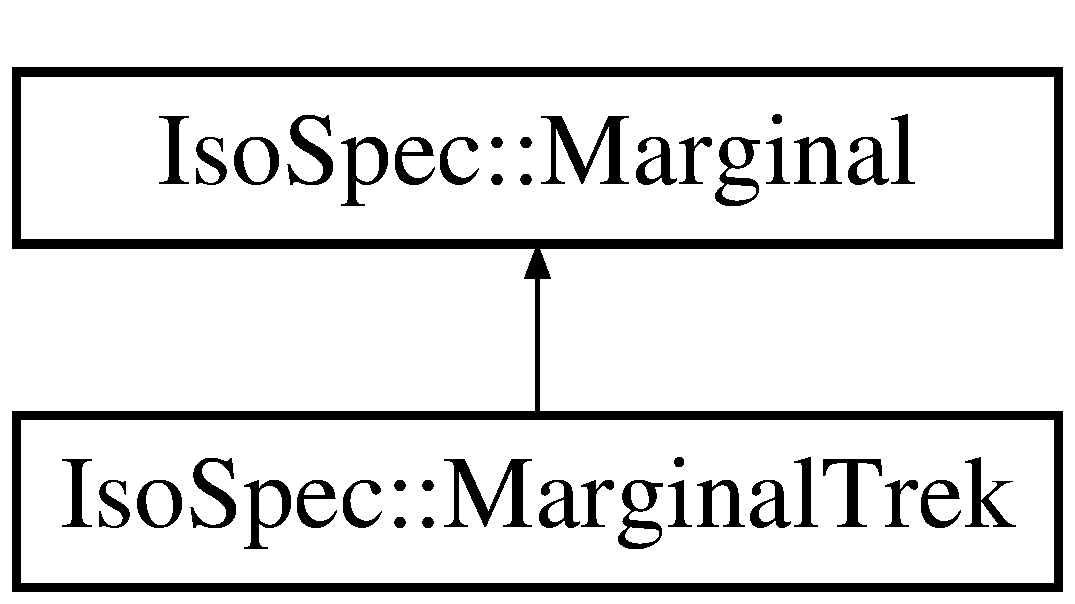
\includegraphics[height=2.000000cm]{class_iso_spec_1_1_marginal_trek}
\end{center}
\end{figure}
\subsection*{Public Member Functions}
\begin{DoxyCompactItemize}
\item 
\mbox{\hyperlink{class_iso_spec_1_1_marginal_trek_a83e70d522174e4e6724116941fd9c99e}{Marginal\+Trek}} (\mbox{\hyperlink{class_iso_spec_1_1_marginal}{Marginal}} \&\&m, int tab\+Size=1000, int hash\+Size=1000)
\begin{DoxyCompactList}\small\item\em Move constructor\+: specializes the \mbox{\hyperlink{class_iso_spec_1_1_marginal}{Marginal}} class. \end{DoxyCompactList}\item 
bool \mbox{\hyperlink{class_iso_spec_1_1_marginal_trek_a4db6041328b818d123a017dda3c8b8ae}{probe\+Configuration\+Idx}} (int idx)
\begin{DoxyCompactList}\small\item\em Check if the table of computed subisotopologues does not have to be extended. \end{DoxyCompactList}\item 
int \mbox{\hyperlink{class_iso_spec_1_1_marginal_trek_a04f3e495a805a3ea242059c963c5b129}{process\+Until\+Cutoff}} (double cutoff)
\begin{DoxyCompactList}\small\item\em Calculate subisotopologues with probability above or equal to the cut-\/off. \end{DoxyCompactList}\item 
\mbox{\Hypertarget{class_iso_spec_1_1_marginal_trek_a802aa5dfd06d560b4f867240bb6c9d10}\label{class_iso_spec_1_1_marginal_trek_a802aa5dfd06d560b4f867240bb6c9d10}} 
const std\+::vector$<$ double $>$ \& {\bfseries conf\+\_\+lprobs} () const
\item 
\mbox{\Hypertarget{class_iso_spec_1_1_marginal_trek_a8b31b886749c0bb07756ae367a4c31cd}\label{class_iso_spec_1_1_marginal_trek_a8b31b886749c0bb07756ae367a4c31cd}} 
const std\+::vector$<$ double $>$ \& {\bfseries conf\+\_\+masses} () const
\item 
\mbox{\Hypertarget{class_iso_spec_1_1_marginal_trek_a05df43d45dda1a7f80b711eec016c40c}\label{class_iso_spec_1_1_marginal_trek_a05df43d45dda1a7f80b711eec016c40c}} 
const std\+::vector$<$ int $\ast$ $>$ \& {\bfseries confs} () const
\end{DoxyCompactItemize}
\subsection*{Additional Inherited Members}


\subsection{Detailed Description}
The marginal distribution class (a subisotopologue). 

Definition at line 141 of file marginal\+Trek++.\+h.



\subsection{Constructor \& Destructor Documentation}
\mbox{\Hypertarget{class_iso_spec_1_1_marginal_trek_a83e70d522174e4e6724116941fd9c99e}\label{class_iso_spec_1_1_marginal_trek_a83e70d522174e4e6724116941fd9c99e}} 
\index{Iso\+Spec\+::\+Marginal\+Trek@{Iso\+Spec\+::\+Marginal\+Trek}!Marginal\+Trek@{Marginal\+Trek}}
\index{Marginal\+Trek@{Marginal\+Trek}!Iso\+Spec\+::\+Marginal\+Trek@{Iso\+Spec\+::\+Marginal\+Trek}}
\subsubsection{\texorpdfstring{Marginal\+Trek()}{MarginalTrek()}}
{\footnotesize\ttfamily Iso\+Spec\+::\+Marginal\+Trek\+::\+Marginal\+Trek (\begin{DoxyParamCaption}\item[{\mbox{\hyperlink{class_iso_spec_1_1_marginal}{Marginal}} \&\&}]{m,  }\item[{int}]{tab\+Size = {\ttfamily 1000},  }\item[{int}]{hash\+Size = {\ttfamily 1000} }\end{DoxyParamCaption})}



Move constructor\+: specializes the \mbox{\hyperlink{class_iso_spec_1_1_marginal}{Marginal}} class. 


\begin{DoxyParams}{Parameters}
{\em tab\+Size} & The size of the table used to store configurations in the allocator. \\
\hline
{\em hash\+Size} & The size of the hash table used to store visited subisotopologues. \\
\hline
\end{DoxyParams}


Definition at line 256 of file marginal\+Trek++.\+cpp.



\subsection{Member Function Documentation}
\mbox{\Hypertarget{class_iso_spec_1_1_marginal_trek_a4db6041328b818d123a017dda3c8b8ae}\label{class_iso_spec_1_1_marginal_trek_a4db6041328b818d123a017dda3c8b8ae}} 
\index{Iso\+Spec\+::\+Marginal\+Trek@{Iso\+Spec\+::\+Marginal\+Trek}!probe\+Configuration\+Idx@{probe\+Configuration\+Idx}}
\index{probe\+Configuration\+Idx@{probe\+Configuration\+Idx}!Iso\+Spec\+::\+Marginal\+Trek@{Iso\+Spec\+::\+Marginal\+Trek}}
\subsubsection{\texorpdfstring{probe\+Configuration\+Idx()}{probeConfigurationIdx()}}
{\footnotesize\ttfamily bool Iso\+Spec\+::\+Marginal\+Trek\+::probe\+Configuration\+Idx (\begin{DoxyParamCaption}\item[{int}]{idx }\end{DoxyParamCaption})\hspace{0.3cm}{\ttfamily [inline]}}



Check if the table of computed subisotopologues does not have to be extended. 

This function checks if the idx-\/th most probable subisotopologue was memoized and if not, computes it and memoizes it.


\begin{DoxyParams}{Parameters}
{\em idx} & The number of the idx-\/th most probable subisotopologue. \\
\hline
\end{DoxyParams}
\begin{DoxyReturn}{Returns}
Returns false if it the provided idx exceeds the total number of subisotopologues. 
\end{DoxyReturn}


Definition at line 179 of file marginal\+Trek++.\+h.

\mbox{\Hypertarget{class_iso_spec_1_1_marginal_trek_a04f3e495a805a3ea242059c963c5b129}\label{class_iso_spec_1_1_marginal_trek_a04f3e495a805a3ea242059c963c5b129}} 
\index{Iso\+Spec\+::\+Marginal\+Trek@{Iso\+Spec\+::\+Marginal\+Trek}!process\+Until\+Cutoff@{process\+Until\+Cutoff}}
\index{process\+Until\+Cutoff@{process\+Until\+Cutoff}!Iso\+Spec\+::\+Marginal\+Trek@{Iso\+Spec\+::\+Marginal\+Trek}}
\subsubsection{\texorpdfstring{process\+Until\+Cutoff()}{processUntilCutoff()}}
{\footnotesize\ttfamily int Iso\+Spec\+::\+Marginal\+Trek\+::process\+Until\+Cutoff (\begin{DoxyParamCaption}\item[{double}]{cutoff }\end{DoxyParamCaption})}



Calculate subisotopologues with probability above or equal to the cut-\/off. 


\begin{DoxyParams}{Parameters}
{\em cutoff} & The probability cut-\/off \\
\hline
\end{DoxyParams}
\begin{DoxyReturn}{Returns}
The number of the last subisotopologue above the cut-\/off. 
\end{DoxyReturn}


Definition at line 333 of file marginal\+Trek++.\+cpp.



The documentation for this class was generated from the following files\+:\begin{DoxyCompactItemize}
\item 
/\+Users/matteo/\+Projects/isospec/\+Iso\+Spec/\+Iso\+Spec++/marginal\+Trek++.\+h\item 
/\+Users/matteo/\+Projects/isospec/\+Iso\+Spec/\+Iso\+Spec++/marginal\+Trek++.\+cpp\end{DoxyCompactItemize}

\hypertarget{class_iso_spec_1_1_order_marginals_by_size_decresing}{}\section{Iso\+Spec\+:\+:Order\+Marginals\+By\+Size\+Decresing Class Reference}
\label{class_iso_spec_1_1_order_marginals_by_size_decresing}\index{Iso\+Spec\+::\+Order\+Marginals\+By\+Size\+Decresing@{Iso\+Spec\+::\+Order\+Marginals\+By\+Size\+Decresing}}
\subsection*{Public Member Functions}
\begin{DoxyCompactItemize}
\item 
\mbox{\Hypertarget{class_iso_spec_1_1_order_marginals_by_size_decresing_a2530a398df14766242b936e5c83e0f37}\label{class_iso_spec_1_1_order_marginals_by_size_decresing_a2530a398df14766242b936e5c83e0f37}} 
{\bfseries Order\+Marginals\+By\+Size\+Decresing} (\mbox{\hyperlink{class_iso_spec_1_1_precalculated_marginal}{Precalculated\+Marginal}} const $\ast$const $\ast$\+\_\+T)
\item 
\mbox{\Hypertarget{class_iso_spec_1_1_order_marginals_by_size_decresing_a43312dd35580f579c9e64b32e06edb63}\label{class_iso_spec_1_1_order_marginals_by_size_decresing_a43312dd35580f579c9e64b32e06edb63}} 
bool {\bfseries operator()} (int m1, int m2)
\end{DoxyCompactItemize}


\subsection{Detailed Description}


Definition at line 128 of file operators.\+h.



The documentation for this class was generated from the following file\+:\begin{DoxyCompactItemize}
\item 
/\+Users/matteo/\+Projects/isospec/\+Iso\+Spec/\+Iso\+Spec++/operators.\+h\end{DoxyCompactItemize}

\hypertarget{class_iso_spec_1_1_precalculated_marginal}{}\section{Iso\+Spec\+:\+:Precalculated\+Marginal Class Reference}
\label{class_iso_spec_1_1_precalculated_marginal}\index{Iso\+Spec\+::\+Precalculated\+Marginal@{Iso\+Spec\+::\+Precalculated\+Marginal}}


Precalculated \mbox{\hyperlink{class_iso_spec_1_1_marginal}{Marginal}} class.  




{\ttfamily \#include $<$marginal\+Trek++.\+h$>$}

Inheritance diagram for Iso\+Spec\+:\+:Precalculated\+Marginal\+:\begin{figure}[H]
\begin{center}
\leavevmode
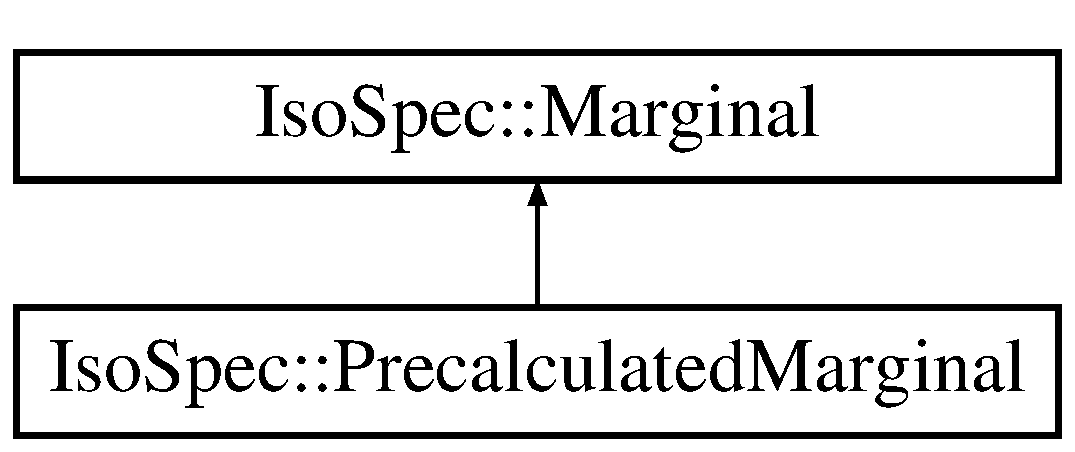
\includegraphics[height=2.000000cm]{class_iso_spec_1_1_precalculated_marginal}
\end{center}
\end{figure}
\subsection*{Public Member Functions}
\begin{DoxyCompactItemize}
\item 
\mbox{\hyperlink{class_iso_spec_1_1_precalculated_marginal_acb84bd7ba582847655c55bd64d64463e}{Precalculated\+Marginal}} (\mbox{\hyperlink{class_iso_spec_1_1_marginal}{Marginal}} \&\&m, double l\+Cut\+Off, bool sort=true, int tab\+Size=1000, int hash\+Size=1000)
\begin{DoxyCompactList}\small\item\em The move constructor (disowns the \mbox{\hyperlink{class_iso_spec_1_1_marginal}{Marginal}}). \end{DoxyCompactList}\item 
\mbox{\Hypertarget{class_iso_spec_1_1_precalculated_marginal_a6b7b30cfe90ffba1d2c9d2f0d87107d8}\label{class_iso_spec_1_1_precalculated_marginal_a6b7b30cfe90ffba1d2c9d2f0d87107d8}} 
virtual \mbox{\hyperlink{class_iso_spec_1_1_precalculated_marginal_a6b7b30cfe90ffba1d2c9d2f0d87107d8}{$\sim$\+Precalculated\+Marginal}} ()
\begin{DoxyCompactList}\small\item\em Destructor. \end{DoxyCompactList}\item 
bool \mbox{\hyperlink{class_iso_spec_1_1_precalculated_marginal_a942b30ace039f80c50125360be4ed4d2}{in\+Range}} (unsigned int idx) const
\begin{DoxyCompactList}\small\item\em Is there a subisotopologue with a given number? \end{DoxyCompactList}\item 
const double \& \mbox{\hyperlink{class_iso_spec_1_1_precalculated_marginal_a07eee6d60635c9c1d6f92c181994e06a}{get\+\_\+l\+Prob}} (int idx) const
\begin{DoxyCompactList}\small\item\em Get the log-\/probability of the idx-\/th subisotopologue. \end{DoxyCompactList}\item 
const double \& \mbox{\hyperlink{class_iso_spec_1_1_precalculated_marginal_a7a38a567eadf16fa2ad41e81c8f55c02}{get\+\_\+e\+Prob}} (int idx) const
\begin{DoxyCompactList}\small\item\em Get the probability of the idx-\/th subisotopologue. \end{DoxyCompactList}\item 
const double \& \mbox{\hyperlink{class_iso_spec_1_1_precalculated_marginal_ada12caa2e195c1a16c5158a428ea3ed2}{get\+\_\+mass}} (int idx) const
\begin{DoxyCompactList}\small\item\em Get the mass of the idx-\/th subisotopologue. \end{DoxyCompactList}\item 
const double $\ast$ \mbox{\hyperlink{class_iso_spec_1_1_precalculated_marginal_af5d01500c7efb8cba57399ba11fc7124}{get\+\_\+l\+Probs\+\_\+ptr}} () const
\begin{DoxyCompactList}\small\item\em Get the table of the log-\/probabilities of subisotopologues. \end{DoxyCompactList}\item 
const double $\ast$ \mbox{\hyperlink{class_iso_spec_1_1_precalculated_marginal_a9a768b90299ea16c447a392dbe1123b5}{get\+\_\+masses\+\_\+ptr}} () const
\begin{DoxyCompactList}\small\item\em Get the table of the masses of subisotopologues. \end{DoxyCompactList}\item 
const Conf \& \mbox{\hyperlink{class_iso_spec_1_1_precalculated_marginal_a3ecbbf1263a274cc8e3bc71cd96f0bff}{get\+\_\+conf}} (int idx) const
\begin{DoxyCompactList}\small\item\em Get the counts of isotopes that define the subisotopologue. \end{DoxyCompactList}\item 
unsigned int \mbox{\hyperlink{class_iso_spec_1_1_precalculated_marginal_a0dbf1ec53eac9953a354c11e1b0803f9}{get\+\_\+no\+\_\+confs}} () const
\begin{DoxyCompactList}\small\item\em Get the number of precomputed subisotopologues. \end{DoxyCompactList}\end{DoxyCompactItemize}
\subsection*{Protected Attributes}
\begin{DoxyCompactItemize}
\item 
\mbox{\Hypertarget{class_iso_spec_1_1_precalculated_marginal_adaba0751ea134b2cbd6c3fdf67c327ea}\label{class_iso_spec_1_1_precalculated_marginal_adaba0751ea134b2cbd6c3fdf67c327ea}} 
std\+::vector$<$ Conf $>$ {\bfseries configurations}
\item 
\mbox{\Hypertarget{class_iso_spec_1_1_precalculated_marginal_a1197bed742b2139243e9dc71cb8fcdfc}\label{class_iso_spec_1_1_precalculated_marginal_a1197bed742b2139243e9dc71cb8fcdfc}} 
Conf $\ast$ {\bfseries confs}
\item 
\mbox{\Hypertarget{class_iso_spec_1_1_precalculated_marginal_ad82d7aef36c946ce4f9bbf3ddac70cd1}\label{class_iso_spec_1_1_precalculated_marginal_ad82d7aef36c946ce4f9bbf3ddac70cd1}} 
unsigned int {\bfseries no\+\_\+confs}
\item 
\mbox{\Hypertarget{class_iso_spec_1_1_precalculated_marginal_a94e78eba4ae89c0d6c811d7bc0085684}\label{class_iso_spec_1_1_precalculated_marginal_a94e78eba4ae89c0d6c811d7bc0085684}} 
double $\ast$ {\bfseries masses}
\item 
\mbox{\Hypertarget{class_iso_spec_1_1_precalculated_marginal_afd5a4a7b094038f66eda31c6827a66f9}\label{class_iso_spec_1_1_precalculated_marginal_afd5a4a7b094038f66eda31c6827a66f9}} 
double $\ast$ {\bfseries l\+Probs}
\item 
\mbox{\Hypertarget{class_iso_spec_1_1_precalculated_marginal_abf3e9faabf5011f75cfb8e89cb3cdcca}\label{class_iso_spec_1_1_precalculated_marginal_abf3e9faabf5011f75cfb8e89cb3cdcca}} 
double $\ast$ {\bfseries e\+Probs}
\item 
\mbox{\Hypertarget{class_iso_spec_1_1_precalculated_marginal_add0495cfc67fd8b9757b93b07d47e6cf}\label{class_iso_spec_1_1_precalculated_marginal_add0495cfc67fd8b9757b93b07d47e6cf}} 
\mbox{\hyperlink{class_iso_spec_1_1_allocator}{Allocator}}$<$ int $>$ {\bfseries allocator}
\end{DoxyCompactItemize}


\subsection{Detailed Description}
Precalculated \mbox{\hyperlink{class_iso_spec_1_1_marginal}{Marginal}} class. 

This class serves to calculate a set of isotopologues that is defined by the minimal probability threshold.

This works faster than if you did not know the threshold. If you have no idea about the threshold, you would need to call us, to change encode the layered version of the marginal. 

Definition at line 213 of file marginal\+Trek++.\+h.



\subsection{Constructor \& Destructor Documentation}
\mbox{\Hypertarget{class_iso_spec_1_1_precalculated_marginal_acb84bd7ba582847655c55bd64d64463e}\label{class_iso_spec_1_1_precalculated_marginal_acb84bd7ba582847655c55bd64d64463e}} 
\index{Iso\+Spec\+::\+Precalculated\+Marginal@{Iso\+Spec\+::\+Precalculated\+Marginal}!Precalculated\+Marginal@{Precalculated\+Marginal}}
\index{Precalculated\+Marginal@{Precalculated\+Marginal}!Iso\+Spec\+::\+Precalculated\+Marginal@{Iso\+Spec\+::\+Precalculated\+Marginal}}
\subsubsection{\texorpdfstring{Precalculated\+Marginal()}{PrecalculatedMarginal()}}
{\footnotesize\ttfamily Iso\+Spec\+::\+Precalculated\+Marginal\+::\+Precalculated\+Marginal (\begin{DoxyParamCaption}\item[{\mbox{\hyperlink{class_iso_spec_1_1_marginal}{Marginal}} \&\&}]{m,  }\item[{double}]{l\+Cut\+Off,  }\item[{bool}]{sort = {\ttfamily true},  }\item[{int}]{tab\+Size = {\ttfamily 1000},  }\item[{int}]{hash\+Size = {\ttfamily 1000} }\end{DoxyParamCaption})}



The move constructor (disowns the \mbox{\hyperlink{class_iso_spec_1_1_marginal}{Marginal}}). 

This constructor memoizes all subisotopologues with log-\/probability above the provided threshold l\+Cut\+Off 
\begin{DoxyParams}{Parameters}
{\em \mbox{\hyperlink{class_iso_spec_1_1_marginal}{Marginal}}} & An instance of the \mbox{\hyperlink{class_iso_spec_1_1_marginal}{Marginal}} class this class is about to disown. \\
\hline
{\em l\+Cut\+Off} & The lower limit on the log-\/probability of the precomputed subisotopologues. \\
\hline
{\em sort} & Should the subisotopologues be stored with descending probability ? \\
\hline
\end{DoxyParams}
\begin{DoxyReturn}{Returns}
An instance of the \mbox{\hyperlink{class_iso_spec_1_1_precalculated_marginal}{Precalculated\+Marginal}} class. 
\end{DoxyReturn}


Definition at line 362 of file marginal\+Trek++.\+cpp.



\subsection{Member Function Documentation}
\mbox{\Hypertarget{class_iso_spec_1_1_precalculated_marginal_a3ecbbf1263a274cc8e3bc71cd96f0bff}\label{class_iso_spec_1_1_precalculated_marginal_a3ecbbf1263a274cc8e3bc71cd96f0bff}} 
\index{Iso\+Spec\+::\+Precalculated\+Marginal@{Iso\+Spec\+::\+Precalculated\+Marginal}!get\+\_\+conf@{get\+\_\+conf}}
\index{get\+\_\+conf@{get\+\_\+conf}!Iso\+Spec\+::\+Precalculated\+Marginal@{Iso\+Spec\+::\+Precalculated\+Marginal}}
\subsubsection{\texorpdfstring{get\+\_\+conf()}{get\_conf()}}
{\footnotesize\ttfamily const Conf\& Iso\+Spec\+::\+Precalculated\+Marginal\+::get\+\_\+conf (\begin{DoxyParamCaption}\item[{int}]{idx }\end{DoxyParamCaption}) const\hspace{0.3cm}{\ttfamily [inline]}}



Get the counts of isotopes that define the subisotopologue. 


\begin{DoxyParams}{Parameters}
{\em idx} & The number of the considered subisotopologue. \\
\hline
\end{DoxyParams}
\begin{DoxyReturn}{Returns}
The counts of isotopes that define the subisotopologue. 
\end{DoxyReturn}


Definition at line 288 of file marginal\+Trek++.\+h.

\mbox{\Hypertarget{class_iso_spec_1_1_precalculated_marginal_a7a38a567eadf16fa2ad41e81c8f55c02}\label{class_iso_spec_1_1_precalculated_marginal_a7a38a567eadf16fa2ad41e81c8f55c02}} 
\index{Iso\+Spec\+::\+Precalculated\+Marginal@{Iso\+Spec\+::\+Precalculated\+Marginal}!get\+\_\+e\+Prob@{get\+\_\+e\+Prob}}
\index{get\+\_\+e\+Prob@{get\+\_\+e\+Prob}!Iso\+Spec\+::\+Precalculated\+Marginal@{Iso\+Spec\+::\+Precalculated\+Marginal}}
\subsubsection{\texorpdfstring{get\+\_\+e\+Prob()}{get\_eProb()}}
{\footnotesize\ttfamily const double\& Iso\+Spec\+::\+Precalculated\+Marginal\+::get\+\_\+e\+Prob (\begin{DoxyParamCaption}\item[{int}]{idx }\end{DoxyParamCaption}) const\hspace{0.3cm}{\ttfamily [inline]}}



Get the probability of the idx-\/th subisotopologue. 


\begin{DoxyParams}{Parameters}
{\em idx} & The number of the considered subisotopologue. \\
\hline
\end{DoxyParams}
\begin{DoxyReturn}{Returns}
The probability of the idx-\/th subisotopologue. 
\end{DoxyReturn}


Definition at line 261 of file marginal\+Trek++.\+h.

\mbox{\Hypertarget{class_iso_spec_1_1_precalculated_marginal_a07eee6d60635c9c1d6f92c181994e06a}\label{class_iso_spec_1_1_precalculated_marginal_a07eee6d60635c9c1d6f92c181994e06a}} 
\index{Iso\+Spec\+::\+Precalculated\+Marginal@{Iso\+Spec\+::\+Precalculated\+Marginal}!get\+\_\+l\+Prob@{get\+\_\+l\+Prob}}
\index{get\+\_\+l\+Prob@{get\+\_\+l\+Prob}!Iso\+Spec\+::\+Precalculated\+Marginal@{Iso\+Spec\+::\+Precalculated\+Marginal}}
\subsubsection{\texorpdfstring{get\+\_\+l\+Prob()}{get\_lProb()}}
{\footnotesize\ttfamily const double\& Iso\+Spec\+::\+Precalculated\+Marginal\+::get\+\_\+l\+Prob (\begin{DoxyParamCaption}\item[{int}]{idx }\end{DoxyParamCaption}) const\hspace{0.3cm}{\ttfamily [inline]}}



Get the log-\/probability of the idx-\/th subisotopologue. 


\begin{DoxyParams}{Parameters}
{\em idx} & The number of the considered subisotopologue. \\
\hline
\end{DoxyParams}
\begin{DoxyReturn}{Returns}
The log-\/probability of the idx-\/th subisotopologue. 
\end{DoxyReturn}


Definition at line 254 of file marginal\+Trek++.\+h.

\mbox{\Hypertarget{class_iso_spec_1_1_precalculated_marginal_af5d01500c7efb8cba57399ba11fc7124}\label{class_iso_spec_1_1_precalculated_marginal_af5d01500c7efb8cba57399ba11fc7124}} 
\index{Iso\+Spec\+::\+Precalculated\+Marginal@{Iso\+Spec\+::\+Precalculated\+Marginal}!get\+\_\+l\+Probs\+\_\+ptr@{get\+\_\+l\+Probs\+\_\+ptr}}
\index{get\+\_\+l\+Probs\+\_\+ptr@{get\+\_\+l\+Probs\+\_\+ptr}!Iso\+Spec\+::\+Precalculated\+Marginal@{Iso\+Spec\+::\+Precalculated\+Marginal}}
\subsubsection{\texorpdfstring{get\+\_\+l\+Probs\+\_\+ptr()}{get\_lProbs\_ptr()}}
{\footnotesize\ttfamily const double$\ast$ Iso\+Spec\+::\+Precalculated\+Marginal\+::get\+\_\+l\+Probs\+\_\+ptr (\begin{DoxyParamCaption}{ }\end{DoxyParamCaption}) const\hspace{0.3cm}{\ttfamily [inline]}}



Get the table of the log-\/probabilities of subisotopologues. 

\begin{DoxyReturn}{Returns}
Pointer to the first element in the table storing log-\/probabilities of subisotopologues. 
\end{DoxyReturn}


Definition at line 274 of file marginal\+Trek++.\+h.

\mbox{\Hypertarget{class_iso_spec_1_1_precalculated_marginal_ada12caa2e195c1a16c5158a428ea3ed2}\label{class_iso_spec_1_1_precalculated_marginal_ada12caa2e195c1a16c5158a428ea3ed2}} 
\index{Iso\+Spec\+::\+Precalculated\+Marginal@{Iso\+Spec\+::\+Precalculated\+Marginal}!get\+\_\+mass@{get\+\_\+mass}}
\index{get\+\_\+mass@{get\+\_\+mass}!Iso\+Spec\+::\+Precalculated\+Marginal@{Iso\+Spec\+::\+Precalculated\+Marginal}}
\subsubsection{\texorpdfstring{get\+\_\+mass()}{get\_mass()}}
{\footnotesize\ttfamily const double\& Iso\+Spec\+::\+Precalculated\+Marginal\+::get\+\_\+mass (\begin{DoxyParamCaption}\item[{int}]{idx }\end{DoxyParamCaption}) const\hspace{0.3cm}{\ttfamily [inline]}}



Get the mass of the idx-\/th subisotopologue. 


\begin{DoxyParams}{Parameters}
{\em idx} & The number of the considered subisotopologue. \\
\hline
\end{DoxyParams}
\begin{DoxyReturn}{Returns}
The mass of the idx-\/th subisotopologue. 
\end{DoxyReturn}


Definition at line 268 of file marginal\+Trek++.\+h.

\mbox{\Hypertarget{class_iso_spec_1_1_precalculated_marginal_a9a768b90299ea16c447a392dbe1123b5}\label{class_iso_spec_1_1_precalculated_marginal_a9a768b90299ea16c447a392dbe1123b5}} 
\index{Iso\+Spec\+::\+Precalculated\+Marginal@{Iso\+Spec\+::\+Precalculated\+Marginal}!get\+\_\+masses\+\_\+ptr@{get\+\_\+masses\+\_\+ptr}}
\index{get\+\_\+masses\+\_\+ptr@{get\+\_\+masses\+\_\+ptr}!Iso\+Spec\+::\+Precalculated\+Marginal@{Iso\+Spec\+::\+Precalculated\+Marginal}}
\subsubsection{\texorpdfstring{get\+\_\+masses\+\_\+ptr()}{get\_masses\_ptr()}}
{\footnotesize\ttfamily const double$\ast$ Iso\+Spec\+::\+Precalculated\+Marginal\+::get\+\_\+masses\+\_\+ptr (\begin{DoxyParamCaption}{ }\end{DoxyParamCaption}) const\hspace{0.3cm}{\ttfamily [inline]}}



Get the table of the masses of subisotopologues. 

\begin{DoxyReturn}{Returns}
Pointer to the first element in the table storing masses of subisotopologues. 
\end{DoxyReturn}


Definition at line 280 of file marginal\+Trek++.\+h.

\mbox{\Hypertarget{class_iso_spec_1_1_precalculated_marginal_a0dbf1ec53eac9953a354c11e1b0803f9}\label{class_iso_spec_1_1_precalculated_marginal_a0dbf1ec53eac9953a354c11e1b0803f9}} 
\index{Iso\+Spec\+::\+Precalculated\+Marginal@{Iso\+Spec\+::\+Precalculated\+Marginal}!get\+\_\+no\+\_\+confs@{get\+\_\+no\+\_\+confs}}
\index{get\+\_\+no\+\_\+confs@{get\+\_\+no\+\_\+confs}!Iso\+Spec\+::\+Precalculated\+Marginal@{Iso\+Spec\+::\+Precalculated\+Marginal}}
\subsubsection{\texorpdfstring{get\+\_\+no\+\_\+confs()}{get\_no\_confs()}}
{\footnotesize\ttfamily unsigned int Iso\+Spec\+::\+Precalculated\+Marginal\+::get\+\_\+no\+\_\+confs (\begin{DoxyParamCaption}{ }\end{DoxyParamCaption}) const\hspace{0.3cm}{\ttfamily [inline]}}



Get the number of precomputed subisotopologues. 

\begin{DoxyReturn}{Returns}
The number of precomputed subisotopologues. 
\end{DoxyReturn}


Definition at line 294 of file marginal\+Trek++.\+h.

\mbox{\Hypertarget{class_iso_spec_1_1_precalculated_marginal_a942b30ace039f80c50125360be4ed4d2}\label{class_iso_spec_1_1_precalculated_marginal_a942b30ace039f80c50125360be4ed4d2}} 
\index{Iso\+Spec\+::\+Precalculated\+Marginal@{Iso\+Spec\+::\+Precalculated\+Marginal}!in\+Range@{in\+Range}}
\index{in\+Range@{in\+Range}!Iso\+Spec\+::\+Precalculated\+Marginal@{Iso\+Spec\+::\+Precalculated\+Marginal}}
\subsubsection{\texorpdfstring{in\+Range()}{inRange()}}
{\footnotesize\ttfamily bool Iso\+Spec\+::\+Precalculated\+Marginal\+::in\+Range (\begin{DoxyParamCaption}\item[{unsigned int}]{idx }\end{DoxyParamCaption}) const\hspace{0.3cm}{\ttfamily [inline]}}



Is there a subisotopologue with a given number? 

\begin{DoxyReturn}{Returns}
Returns true if idx does not exceed the number of pre-\/computed configurations. 
\end{DoxyReturn}


Definition at line 247 of file marginal\+Trek++.\+h.



The documentation for this class was generated from the following files\+:\begin{DoxyCompactItemize}
\item 
/\+Users/matteo/\+Projects/isospec/\+Iso\+Spec/\+Iso\+Spec++/marginal\+Trek++.\+h\item 
/\+Users/matteo/\+Projects/isospec/\+Iso\+Spec/\+Iso\+Spec++/marginal\+Trek++.\+cpp\end{DoxyCompactItemize}

\hypertarget{class_iso_spec_1_1_reverse_order}{}\section{Iso\+Spec\+:\+:Reverse\+Order$<$ T $>$ Class Template Reference}
\label{class_iso_spec_1_1_reverse_order}\index{Iso\+Spec\+::\+Reverse\+Order$<$ T $>$@{Iso\+Spec\+::\+Reverse\+Order$<$ T $>$}}
\subsection*{Public Member Functions}
\begin{DoxyCompactItemize}
\item 
\mbox{\Hypertarget{class_iso_spec_1_1_reverse_order_a350cba89162d701a0f0f4cf1e4424e44}\label{class_iso_spec_1_1_reverse_order_a350cba89162d701a0f0f4cf1e4424e44}} 
bool {\bfseries operator()} (const T a, const T b) const
\end{DoxyCompactItemize}


\subsection{Detailed Description}
\subsubsection*{template$<$typename T$>$\newline
class Iso\+Spec\+::\+Reverse\+Order$<$ T $>$}



Definition at line 106 of file operators.\+h.



The documentation for this class was generated from the following file\+:\begin{DoxyCompactItemize}
\item 
/\+Users/matteo/\+Projects/isospec/\+Iso\+Spec/\+Iso\+Spec++/operators.\+h\end{DoxyCompactItemize}

\hypertarget{class_iso_spec_1_1_s_summator}{}\section{Iso\+Spec\+:\+:S\+Summator Class Reference}
\label{class_iso_spec_1_1_s_summator}\index{Iso\+Spec\+::\+S\+Summator@{Iso\+Spec\+::\+S\+Summator}}
\subsection*{Public Member Functions}
\begin{DoxyCompactItemize}
\item 
\mbox{\Hypertarget{class_iso_spec_1_1_s_summator_a5173dbb75fb32ad67bf3abd1ae6f9dc6}\label{class_iso_spec_1_1_s_summator_a5173dbb75fb32ad67bf3abd1ae6f9dc6}} 
{\bfseries S\+Summator} (\mbox{\hyperlink{class_iso_spec_1_1_s_summator}{S\+Summator}} \&other)
\item 
\mbox{\Hypertarget{class_iso_spec_1_1_s_summator_aad1c7ce5e38ce2da7d9e39f43e647402}\label{class_iso_spec_1_1_s_summator_aad1c7ce5e38ce2da7d9e39f43e647402}} 
void {\bfseries add} (double x)
\item 
\mbox{\Hypertarget{class_iso_spec_1_1_s_summator_ab7b2c53b5e9258aa4c7e7707089fbb6a}\label{class_iso_spec_1_1_s_summator_ab7b2c53b5e9258aa4c7e7707089fbb6a}} 
double {\bfseries get} ()
\end{DoxyCompactItemize}


\subsection{Detailed Description}


Definition at line 25 of file summator.\+h.



The documentation for this class was generated from the following file\+:\begin{DoxyCompactItemize}
\item 
/\+Users/matteo/\+Projects/isospec/\+Iso\+Spec/\+Iso\+Spec++/summator.\+h\end{DoxyCompactItemize}

\hypertarget{class_iso_spec_1_1_summator}{}\section{Iso\+Spec\+:\+:Summator Class Reference}
\label{class_iso_spec_1_1_summator}\index{Iso\+Spec\+::\+Summator@{Iso\+Spec\+::\+Summator}}
\subsection*{Public Member Functions}
\begin{DoxyCompactItemize}
\item 
\mbox{\Hypertarget{class_iso_spec_1_1_summator_a1b032359eb84e5788ab31c3ad3932008}\label{class_iso_spec_1_1_summator_a1b032359eb84e5788ab31c3ad3932008}} 
void {\bfseries add} (double what)
\item 
\mbox{\Hypertarget{class_iso_spec_1_1_summator_a87f3249839e99b41d3c16aeed75204fa}\label{class_iso_spec_1_1_summator_a87f3249839e99b41d3c16aeed75204fa}} 
double {\bfseries get} ()
\end{DoxyCompactItemize}


\subsection{Detailed Description}


Definition at line 76 of file summator.\+h.



The documentation for this class was generated from the following file\+:\begin{DoxyCompactItemize}
\item 
/\+Users/matteo/\+Projects/isospec/\+Iso\+Spec/\+Iso\+Spec++/summator.\+h\end{DoxyCompactItemize}

\hypertarget{class_iso_spec_1_1_table_order}{}\section{Iso\+Spec\+:\+:Table\+Order$<$ T $>$ Class Template Reference}
\label{class_iso_spec_1_1_table_order}\index{Iso\+Spec\+::\+Table\+Order$<$ T $>$@{Iso\+Spec\+::\+Table\+Order$<$ T $>$}}
\subsection*{Public Member Functions}
\begin{DoxyCompactItemize}
\item 
\mbox{\Hypertarget{class_iso_spec_1_1_table_order_a82a2474a7990bf0a55e269ea2dabada5}\label{class_iso_spec_1_1_table_order_a82a2474a7990bf0a55e269ea2dabada5}} 
{\bfseries Table\+Order} (const T $\ast$\+\_\+tbl)
\item 
\mbox{\Hypertarget{class_iso_spec_1_1_table_order_a35b990bbb3f8c3ba0551c0938a5145c8}\label{class_iso_spec_1_1_table_order_a35b990bbb3f8c3ba0551c0938a5145c8}} 
bool {\bfseries operator()} (unsigned int i, unsigned int j)
\end{DoxyCompactItemize}


\subsection{Detailed Description}
\subsubsection*{template$<$typename T$>$\newline
class Iso\+Spec\+::\+Table\+Order$<$ T $>$}



Definition at line 113 of file operators.\+h.



The documentation for this class was generated from the following file\+:\begin{DoxyCompactItemize}
\item 
/\+Users/matteo/\+Projects/isospec/\+Iso\+Spec/\+Iso\+Spec++/operators.\+h\end{DoxyCompactItemize}

\hypertarget{class_iso_spec_1_1_tabulator}{}\section{Iso\+Spec\+:\+:Tabulator$<$ T $>$ Class Template Reference}
\label{class_iso_spec_1_1_tabulator}\index{Iso\+Spec\+::\+Tabulator$<$ T $>$@{Iso\+Spec\+::\+Tabulator$<$ T $>$}}
\subsection*{Public Member Functions}
\begin{DoxyCompactItemize}
\item 
\mbox{\Hypertarget{class_iso_spec_1_1_tabulator_a57acb4ba7687ac95916c00fd9cd4f4c7}\label{class_iso_spec_1_1_tabulator_a57acb4ba7687ac95916c00fd9cd4f4c7}} 
{\bfseries Tabulator} (T $\ast$generator, bool get\+\_\+masses, bool get\+\_\+probs, bool get\+\_\+lprobs, bool get\+\_\+confs)
\item 
\mbox{\Hypertarget{class_iso_spec_1_1_tabulator_ae256b348fc6c5d24d540c33094a37df9}\label{class_iso_spec_1_1_tabulator_ae256b348fc6c5d24d540c33094a37df9}} 
double $\ast$ {\bfseries masses} ()
\item 
\mbox{\Hypertarget{class_iso_spec_1_1_tabulator_a486be3022d437b81b4932dd61ca4a0e5}\label{class_iso_spec_1_1_tabulator_a486be3022d437b81b4932dd61ca4a0e5}} 
double $\ast$ {\bfseries lprobs} ()
\item 
\mbox{\Hypertarget{class_iso_spec_1_1_tabulator_a0c572de1f59a3c664c55e55760be2f18}\label{class_iso_spec_1_1_tabulator_a0c572de1f59a3c664c55e55760be2f18}} 
double $\ast$ {\bfseries probs} ()
\item 
\mbox{\Hypertarget{class_iso_spec_1_1_tabulator_a8000f897020376b6a03fb75dafb997f1}\label{class_iso_spec_1_1_tabulator_a8000f897020376b6a03fb75dafb997f1}} 
int $\ast$ {\bfseries confs} ()
\item 
\mbox{\Hypertarget{class_iso_spec_1_1_tabulator_acdbd459f1ec95dfd17cc0617cda02fba}\label{class_iso_spec_1_1_tabulator_acdbd459f1ec95dfd17cc0617cda02fba}} 
size\+\_\+t {\bfseries confs\+\_\+no} ()
\end{DoxyCompactItemize}


\subsection{Detailed Description}
\subsubsection*{template$<$typename T$>$\newline
class Iso\+Spec\+::\+Tabulator$<$ T $>$}



Definition at line 12 of file tabulator.\+h.



The documentation for this class was generated from the following file\+:\begin{DoxyCompactItemize}
\item 
/\+Users/matteo/\+Projects/isospec/\+Iso\+Spec/\+Iso\+Spec++/tabulator.\+h\end{DoxyCompactItemize}

\hypertarget{class_iso_spec_1_1_t_summator}{}\section{Iso\+Spec\+:\+:T\+Summator Class Reference}
\label{class_iso_spec_1_1_t_summator}\index{Iso\+Spec\+::\+T\+Summator@{Iso\+Spec\+::\+T\+Summator}}
\subsection*{Public Member Functions}
\begin{DoxyCompactItemize}
\item 
\mbox{\Hypertarget{class_iso_spec_1_1_t_summator_a5645d3fdac4e35f023fe7a08646dc413}\label{class_iso_spec_1_1_t_summator_a5645d3fdac4e35f023fe7a08646dc413}} 
void {\bfseries add} (double what)
\item 
\mbox{\Hypertarget{class_iso_spec_1_1_t_summator_a0db3add5376aae480fcaa3f489898bd7}\label{class_iso_spec_1_1_t_summator_a0db3add5376aae480fcaa3f489898bd7}} 
double {\bfseries get} ()
\end{DoxyCompactItemize}


\subsection{Detailed Description}


Definition at line 99 of file summator.\+h.



The documentation for this class was generated from the following file\+:\begin{DoxyCompactItemize}
\item 
/\+Users/matteo/\+Projects/isospec/\+Iso\+Spec/\+Iso\+Spec++/summator.\+h\end{DoxyCompactItemize}

%--- End generated contents ---

% Index
\backmatter
\newpage
\phantomsection
\clearemptydoublepage
\addcontentsline{toc}{chapter}{Index}
\printindex

\end{document}
